\documentclass[onecolumn, draftclsnofoot,10pt, compsoc]{article}
\usepackage{graphicx}
\usepackage{url}
\usepackage{lscape}
\usepackage{setspace}
\usepackage{parskip}
\usepackage{geometry}
\usepackage{vhistory}
\geometry{textheight=9.5in, textwidth=7in}
\graphicspath{{Figures/}}

% 1. Fill in these details
\def \CapstoneTeamName{AgBizClimate}
\def \CapstoneTeamNumber{26}
\def \GroupMemberOne{	Thomas Noelcke}
\def \GroupMemberTwo{	Shane Barrantes}
\def \GroupMemberThree{	Shengpei Yuan}
\def \CapstoneProjectName{ Linking Seasonal Weather Data to AgBizClimate\texttrademark}
\def \CapstoneSponsorCompany{ Oregon State University}
\def \CapstoneSponsorPerson{ Clark Seavert}
\def \CapstoneProjectLead{ Sean Hammond}

% 2. Uncomment the appropriate line below so that the document type works
\def \DocType{ Software Design Document
				%Requirements Document
				%Technology Review
				%Design Document
				%Progress Report
				}

\newcommand{\NameSigPair}[1]{\par
\makebox[2.75in][r]{#1} \hfil 	\makebox[3.25in]{\makebox[2.25in]{\hrulefill} \hfill		\makebox[.75in]{\hrulefill}}
\par\vspace{-12pt} \textit{\tiny\noindent
\makebox[2.75in]{} \hfil		\makebox[3.25in]{\makebox[2.25in][r]{Signature} \hfill	\makebox[.75in][r]{Date}}}}
% 3. If the document is not to be signed, uncomment the RENEWcommand below
\renewcommand{\NameSigPair}[1]{#1}

%%%%%%%%%%%%%%%%%%%%%%%%%%%%%%%%%%%%%%%
\begin{document}
\begin{titlepage}
    \pagenumbering{gobble}
    \begin{singlespace}
        \hfill
        % 4. If you have a logo, use this includegraphics command to put it on the coversheet.
        %\includegraphics[height=4cm]{CompanyLogo}
        \par\vspace{.2in}
        \centering
        \scshape{
            \huge CS Capstone \DocType \par
            {\large\today}\par
            \vspace{.5in}
            \textbf{\Huge\CapstoneProjectName}\par
            \vfill
            {\large Prepared for}\par
            \Huge \CapstoneSponsorCompany\par
            \vspace{5pt}
            {\Large\NameSigPair{\CapstoneSponsorPerson}\par}
						{\Large\NameSigPair{\CapstoneProjectLead}\par}
            {\large Prepared by }\par
            Group\CapstoneTeamNumber\par
            % 5. comment out the line below this one if you do not wish to name your team
            %\CapstoneTeamName\par
            \vspace{5pt}
            {\Large
                \NameSigPair{\GroupMemberOne}\par
                \NameSigPair{\GroupMemberTwo}\par
                \NameSigPair{\GroupMemberThree}\par
            }
            \vspace{20pt}
        }
				\begin{versionhistory}
					\vhEntry{1.0}{1.12.17}{\GroupMemberOne|\GroupMemberTwo|\GroupMemberThree}{Preliminary Draft}
				\end{versionhistory}
        \begin{abstract}
					This design document will cover the proposed design of the AgBizClimate\texttrademark project. We will first give a general introduction to the project. This section will provide some context for why we are doing this project and what this project hopes to accomplish. Next we will talk about Architecture design. This section will describe a high level structure for the project. After that we will discuss the data for the project and how it will be structured. Then we will discuss in detail the design of each component in the \textit{AgBizClimate} system. We will then discus the design of each view in the user interface. Finally, we will provide a requirements matrix which will show how each component fulfills the functional requirements outlined in the requirements document.
        \end{abstract}
    \end{singlespace}
\end{titlepage}
\newpage
\pagenumbering{arabic}
\tableofcontents
% 7. uncomment this (if applicable). Consider adding a page break.
\listoffigures
\newpage
%\listoftables
\clearpage

% 8. now you write!
\section{Introduction}

		\subsection{Purpose}
			The purpose of this Software Design Description (SDD) is to describe the architecture and system design of the \textit{AgBizClimate} project. This document will provide a high level design for the \textit{AgBizClimate} short term climate tool. This document will also provide a detailed description of the design of the data for this project. We will also break down each component and discuss the design of each component in detail. After that we will discuss the design of each view in the user interface. Finally, we will have a requirements matrix. The requirements matrix will show how each component fulfills the functional requirements for this project.
			This document is intended for the project owners and software developers of the \textit{AgBizClimate} system. This document is intended to be a guide for the implementation of the \textit{AgBizClimate} short term climate tool.

		\subsection{Overview}
			Seasonal climate is one of the essential factors that affects agricultural production. As a module of \textit{AgBiz Logic}, \textit{AgBizClimate} delivers essential information about climate change to farmers, and help professionals to develop management pathways that best fit their operations under a changing climate. This project aims to link the crucial seasonal climate data from the Northwest Climate Toolbox database to \textit{AgBiz Logic} so that it can provide changes in net returns of crop and livestock enterprises through powerful graphics and tables.\\

		\subsection{Scope}
			This project is a part of a much larger AgBiz Logic\texttrademark program. However, the purpose of this project is to add a short term climate tool to the \textit{AgBizClimate} module. This limits the scope of the project to the \textit{AgBizClimate} Module. Additionally, we will only be adding the short term climate data tool as the long term climate data tool already exists.\\

			Currently \textit{AgBizClimate} has a long-term climate tool but no such tool exists for short term climate data. We will implement a tool to extract short-term climate data from the Northwest Climate Toolbox database, display it to the user and allow the user to adjust crop and livestock yields or quality of products sold and, production inputs. Moreover, a landing tool will be developed to allow users to switch between short-term seasonal tool and long-term climate data tool.\\

		%Please add to this section as you write and use Definitions, Acronyms and Abbreviations.
		\subsection{Definitions, Acronyms and Abbreviations}
			REST - Representational State Transfer, This is a type of architecture that manages the state of the program. This is especially popular in web development.\\
			API- Application Programming Interface. This is a piece of software that allows a connection to another piece of software providing some sort of service.\\
			NWCTB - Northwest Climate Toolbox. This is the database we will be connecting to that will provide the short term climate data we plan to use.\\
			Climate Scenario - This is a theoretical calculation of yields, inputs and of the overall budget for one situation based on the climate data.\\
			SQL Database - This is a relational database that allows for storing and accessing data.\\
			NOSQL Database - This is a non-relational database that allows for data storage and data access.\\
			UI - User Interface, This is a piece of software that allows a human to interact with the software. Often this is what the user sees while using software.

			\renewcommand\refname{\vskip -1cm}
		\subsection{References}

		\nocite{*}
    \bibliographystyle{IEEEtran}
    \bibliography{IEEEabrv,References}


\section{System Overview}
	\subsection {Product Functions}
				\textit{AgBizClimate} is a web based decision tool that will allow users to gain specific insight on how localized climate data for the next seven months will affect their crop and livestock yields or quality of products sold and production inputs. The \textit{AgBizClimate} tool will allow users to input their location (state, county) and a budget for the specific crop or livestock enterprise. \textit{AgBizClimate} will select climate data for the next seven months for that location and provide graphical data showing temperature and precipitation. Users will then be able to change yields or quality of product sold by a percentage they think these factors will affect and modify production inputs. Finally the tool will calculate the net returns.\\

	\subsection{User Characteristics}
		\textit{AgBizClimate} users can be split into two subgroups, agricultural producers and climate researchers. The first subgroup, agricultural users who use this product tend to be between fifty and sixty years old of mixed gender. Their educational background ranges from high school to the completion of college. The primary language this group uses is English, but there are some Spanish users as well. Most of the users in this group tend to have novice computational skills. The primary domain for these users is agricultural and business management. Most agricultural producers who use this product are motivated by the potential profit that the decision tool \textit{AgBizClimate} could potentially offer. The second subgroup, climate researchers range from ages twenty to forty and are of mixed gender. The educational background for most climate researchers  exceed the postgraduate level with their primary language being English. These users generally have advanced computational skills and are motivated by the easily accessible climate and weather data.\\

	\subsection{Constraints}
		There are several key constraints that this product has to work within. The first constraint is that we only have access to two data parameters from the North West Climate Tool box, precipitation and temperature. Secondly, we only have access to their data via the NWCTB API which could have additional restrictions such as limited usage per day, mislabeled data, or poor documentation. Thirdly, we don’t have access to any of the hardware that \textit{AgBizClimate} is exists on as it is being managed by a third party. This will prevent us from improving the hardware or cause roadblocks if their servers are having issues. Lastly, we are limited to using the languages Python and JavaScript since we are integrating our product into an already existing project.\\

	\subsection {Assumptions and Dependencies}
		We are assuming that the Northwest Climate Toolbox is a functional API that will allow us to pull location based temperature and precipitation data. This data will most likely come in the form of a text body of which we will then format into a JSON object and store in a MongoDB database for future use. Due to the fact that we are writing an addition to an existing project we do not need to interact with the user budgets as these have already been defined. This fact extends to the calculations portion of the \textit{AgBizClimate} product. Our team will simply be accessing data via the NWCTB API, then format the data, store the data, and hand the data over to the tool while will provide some additional front end support.\\


\section{System Architecture}
	\subsection{Architectural Design}
		Shown Below is the architectural design for the \textit{AgBizClimate} project. This UML diagram shows the high level components of this application. This Diagram also shows how these components will interact.\\

		%insert diagram here. Please don't be a bitch about where you put the diagrm laTex...
		\begin{figure}[htb]
			\begin{center}
				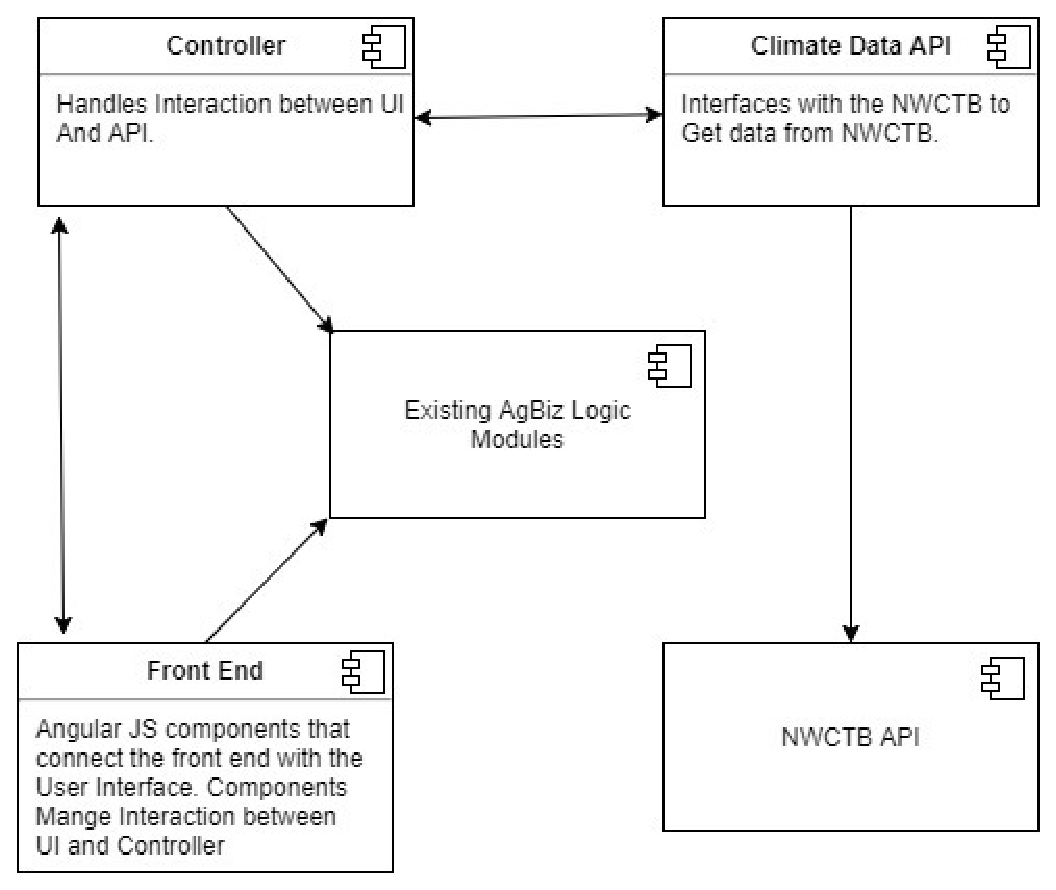
\includegraphics{UMLDiagrams/ArchitectureDesign.eps}
			\end{center}
			\caption{System Architecture Design for \textit{AgBizClimate} project}
			\label{fig:Arch1}
		\end{figure}


	\subsection{Decomposition Description}
		The \textit{AgBizClimate} project can broken down into six components. The six components are the Backend Controller, The Front End Controller, UI, Existing \textit{AgBiz Logic} Modules, Climate Data API, and the NWCTB API. In this section we will describe each models function and how it interacts with the other modules.\\

		\subsubsection{Backend Controller}
			This component is responsible for connecting the dots between the rest of the components. Generally, the backend controller will handle incoming requests from the front end controller and return the requested content. This component will also interface with the existing \textit{AgBiz Logic} modules and Climate Data API so it can provide all the requested information.\\

		\subsubsection{Front End Controller}
			The Front End Controller will act as an interface between the UI, the existing \textit{AgBiz Locic} modules and the Backend Controller. This component will handle UI action made by the user and will use those to make requests to the Backend and existing \textit{AgBiz Logic} Modules. This component will then take the result of these requests and display the relevant information to the user. This component will also handle user inputs such as a button push or clicking on a drop down menu. This component will take these actions and modify the UI to reflect the actions the user preformed.\\

		\subsubsection{UI}
			This is the portion of the application that the user will see and interact with. The primary responsibility of this component is to display information to the user. This component will also be responsible for interacting with the front end Controller to ensure that user actions so the program responds correctly to user action.\\

		\subsubsection{Existing \textit{AgBiz Logic} modules}
			This is not a component but rather a collection of components that already exists as part of the \textit{AgBiz logic} system. We will use these components to preform a variate of actions including, retrieving budget data, managing user information, making modifications to budget data and saving budget data back to the database. We will interface with these component from the Front End Controller to handle budget data. We will also interface with these components from the back end to handle user data.\\


		\subsubsection{Climate Data API}
			The Climate Data API component will interface withe the NWCTB to provide long term forecast data. This component will take requests, with location data, from the Backend controller and will respond with the formatted data from the NWCTB. To do we will interface with the NWCTB API to retrieve the data. Then we will take the data from the NWCTB, parse it into JSON, apply some formatting and pass it back to the Backend. For the purposes of this project this component is only going to interface with the Backend Controller. However in the future this API maybe used by other sections of the application as well.\\

		\subsubsection{NWCTB API}
			The NWCTB API will be our data source for this project. This component will provide the climate data by interfacing with the back end controller. Currently we are not sure how we will interface with the NWCTB as the NWCTB has not responded to our requests for API access.\\

	\subsection{Design Rationale}
		We've chosen to design this system this way in part because of the nature of our system. We need a front end controller to handle the clients interaction with the server because this is a web development project and the front end will be separate from the server. The front end controller will facilitate the communication between the client and the server.\\
		We also chose to use a Backend Controller so we can facilitate the communication between the front end controller and the various components on the backend. This makes the application easier to build, test and maintain. This also allows for one line of communication between the backend and the front end. This is necessary to keep the interactions between the backend code and front end code simple. This allows for large changes to be made to both the front end and the backend with out causing them to impact each other.\\
		We also chose to create the Climate Data API as its own service. We chose to do this because it's easier to test and then the Climate Data API can be reused in future projects and with the other components. If we had built the Climate Data API into the backend controller this would not have been possible.\\
		The NWCTB and Existing \textit{AgBiz Logic} components have already been implemented out side the scope of our project. However, we are still planning to use them in our project. This is why we have created these modules in our design because we will be using them as part of the design of our system but do not want to tightly couple our project with these existing components.\\
		More generally the components in our system use the REST API architecture type. We chose to do this because it allows for flexible reusable modules. The REST API Architecture also allows us to break our application into independent modules that are easier to develop, test and maintain. This division of our application also makes it more scalable allowing our system to keep up with future demand.\\

%in this section we will want to talk about the Climate data and how it will be designed.
%we may also want to breifly mention the user data and budget data. However we will also
%Need to metion that we are not responsible for how those items were designed.
\section{Data Design}
	\subsection{Data Description}
		In this section we will discuss the design of the data required for this system. The data needed to implement this system includes the user data, climate scenarios, Budget Data and the climate data. It should be noted that this project adds the climate data to the system. User data, climate scenarios and budget data have already been implemented as part of the existing \textit{AgBiz Logic} system. However, since we will be using this data as part of our project I've included their design in this section.\\
		Shown below is the design for the data we will use in this program. In this UML diagram are all the various entities required by this system. Additionally we also show the relationship between different entities. Shown below are the UML diagrams for User Data, Climate Scenarios, Budget Data, Climate Data and Related Entities.\\

\clearpage

		%insert UML Diagrams here.
		\begin{figure}[htb]
			\begin{center}
				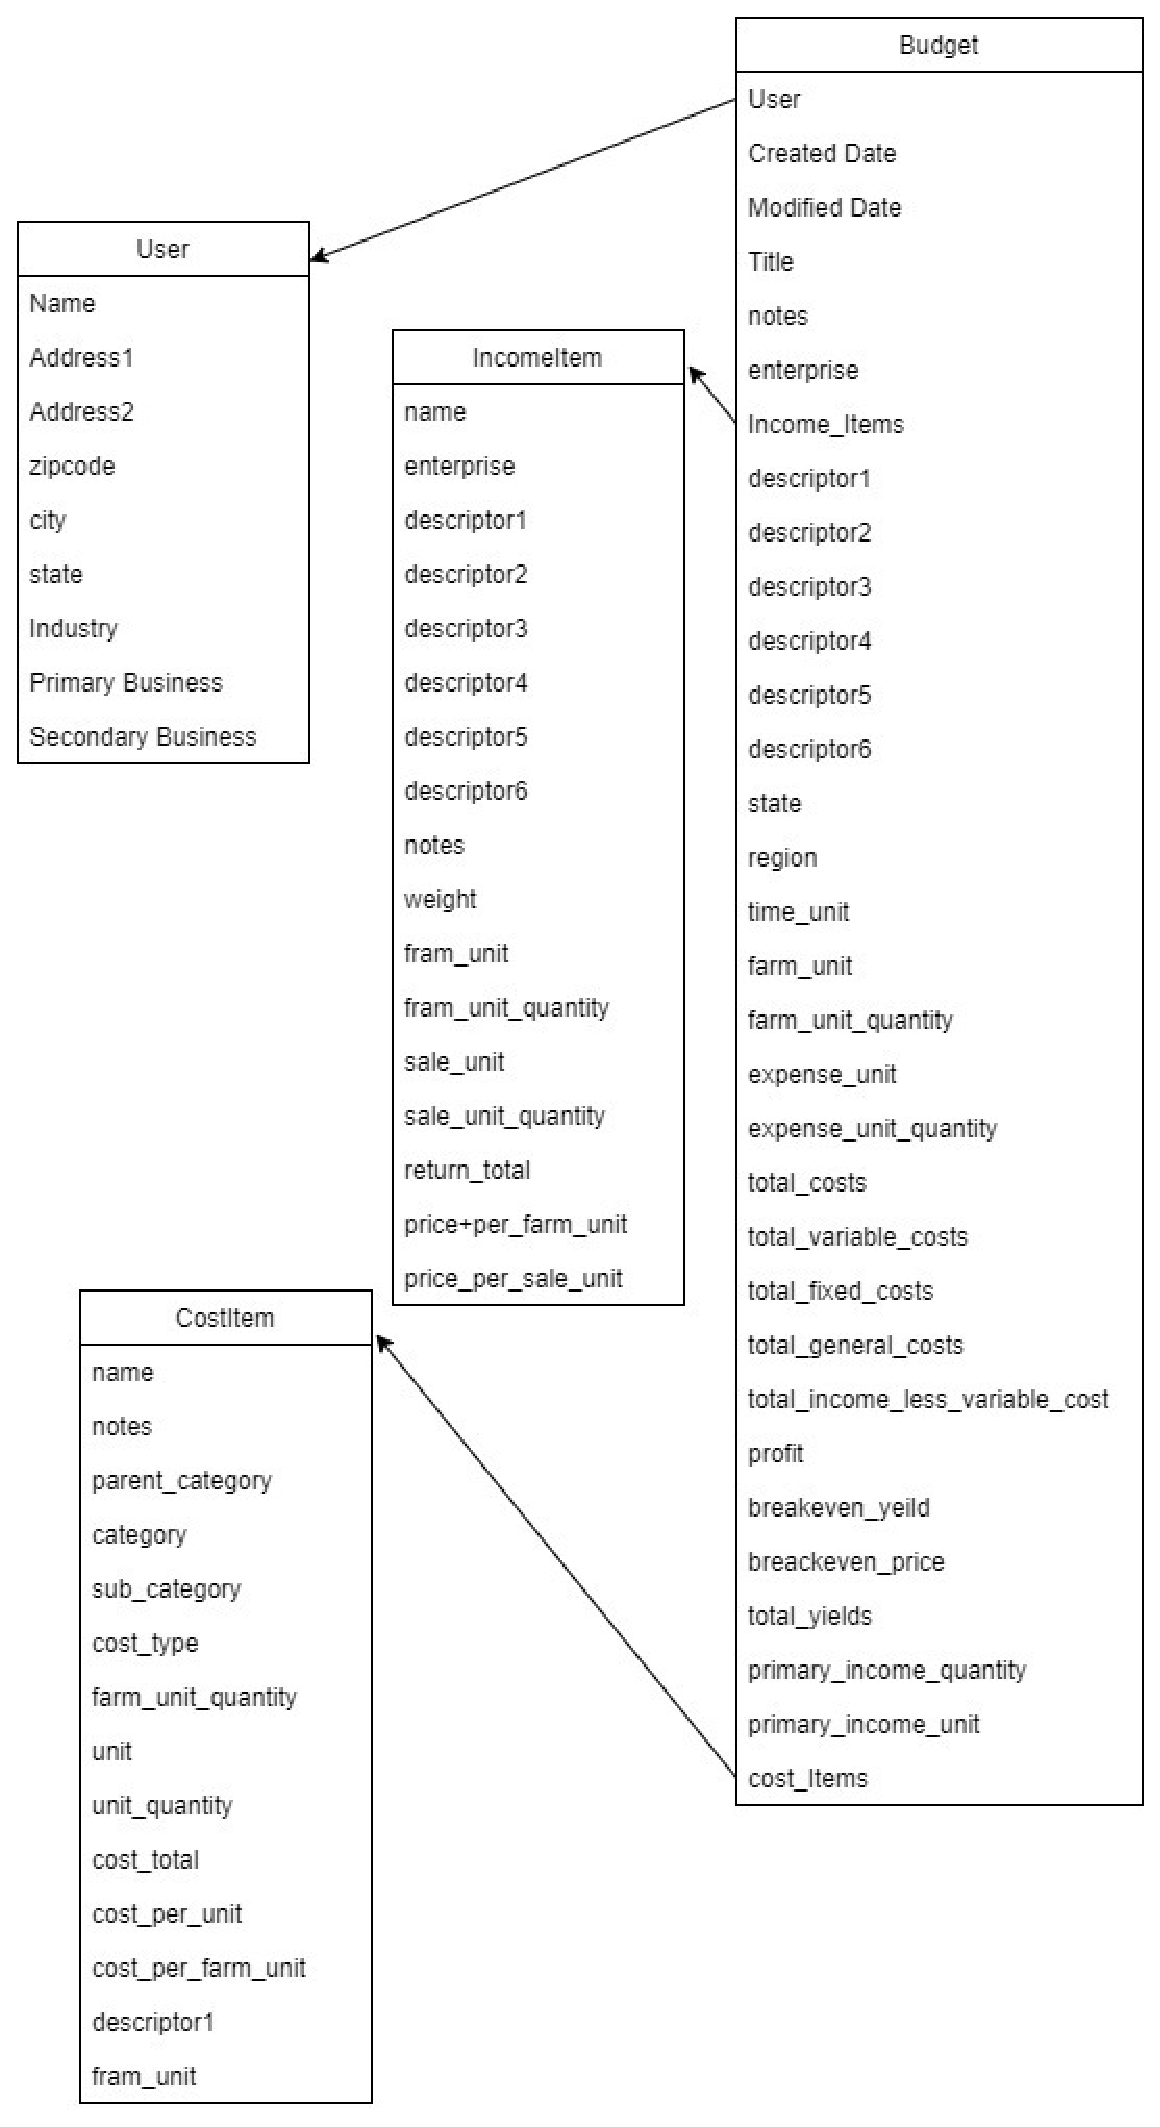
\includegraphics[width=275pt]{UMLDiagrams/UserData.eps}
			\end{center}
			\caption{User Data Currently Implemented in the \textit{AgBiz Logic} project}
			\label{fig:UD1}
		\end{figure}
		\clearpage
		\begin{figure}[htb]
			\begin{center}
				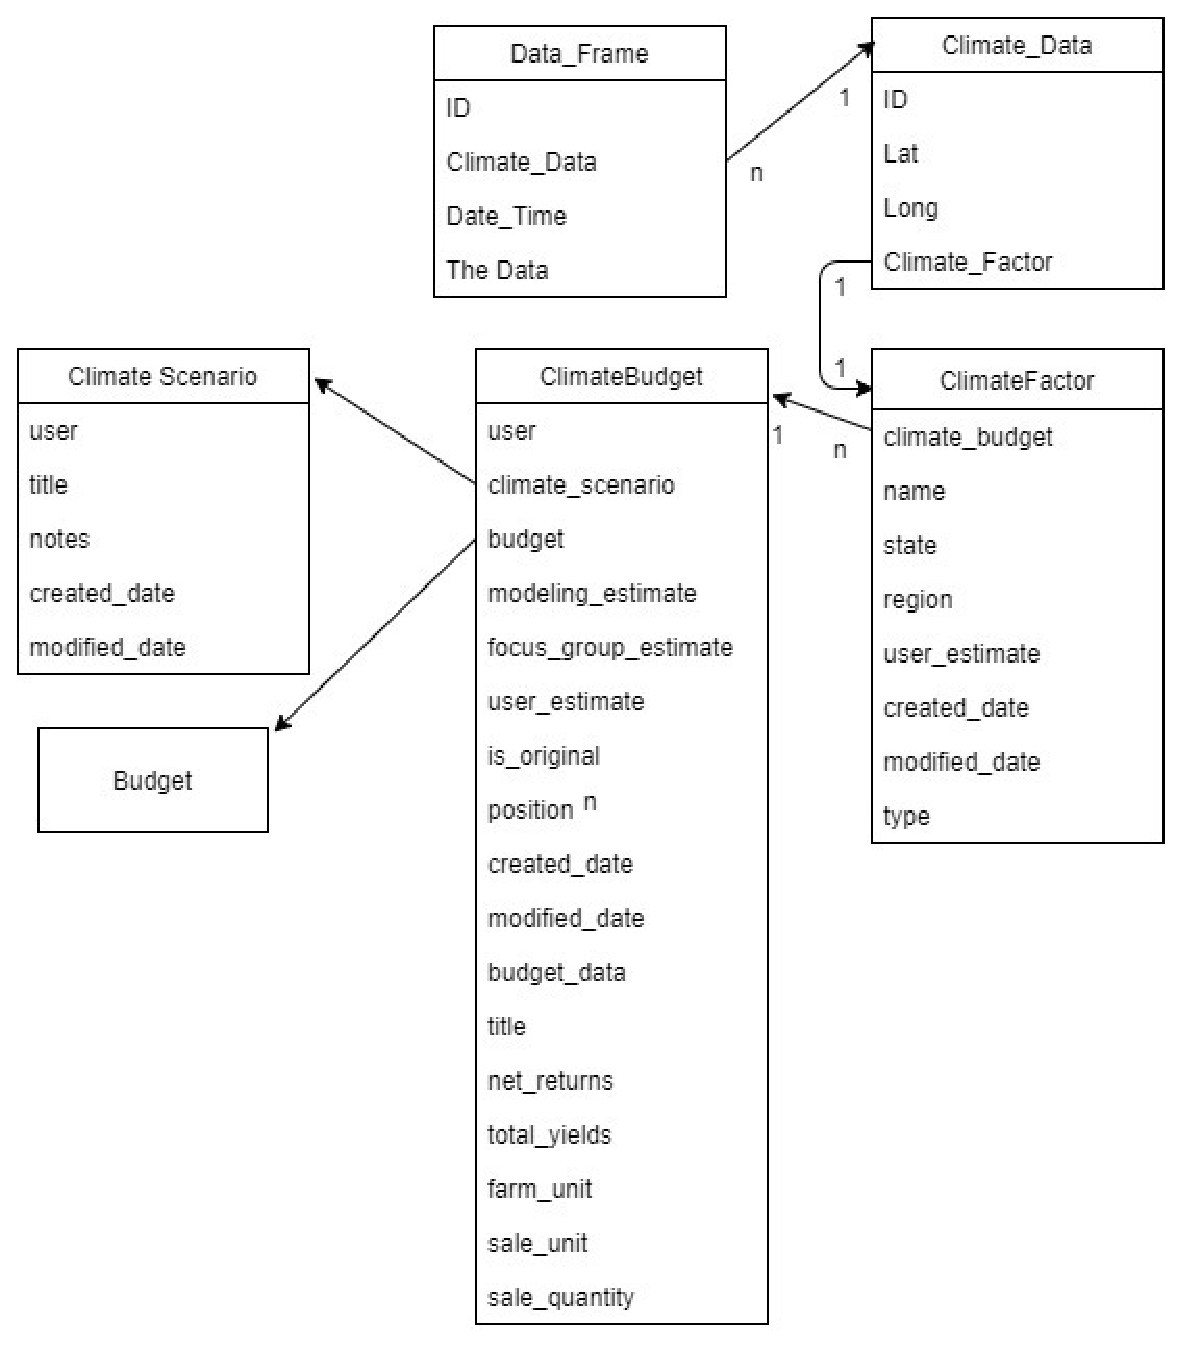
\includegraphics[width=300pt]{UMLDiagrams/ClimateData.eps}
			\end{center}
			\caption{Design For the Climate Data for the \textit{AgBizClimate} project}
			\label{fig:CD1}
		\end{figure}


	\subsection{Data Dictionary}
		In this section we will describe each piece of data and what it represents. We will also discuss possible values for each piece of data.\\
		\subsubsection{User Data}
			In this section we will define the entities and fields that relate to user data and user budgets.\\
			\subsubsection{User}
				This entity represents a user along with the data we will need for each user.\\
				\textbf{Name} - This is a string that stores the user name of a user.\\

				\textbf{Address 1} - This  stores the first line of a users address.\\

				\textbf{Address 2} - This stores the second line of a users address.

				\textbf{zip code} - This stores the zip code for the address the user entered.\\

				\textbf{city} - This stores the name of the city for the address the user entered.\\

				\textbf{state} - This stores the name of the state that the user entered. The state must be a valid US state as climate data is not available for out side the US.\\

				\textbf{Industry} - This stores what industry the user is involved in. Currently the user may choose from two options Agriculture or Non-Agriculture.\\

				\textbf{Primary Business} - This stores what sort of business a user is employed in. For instance if a user were a farmer they would select Producer.\\

				\textbf{Secondary Business} - This is an optional parameter that stores what if any other business that the user may engage in. For instance if a user is a producer but also packages their product them selves they would select packager for this option.\\

			\subsubsection{Budget}
				This entity represents a budget and associated data. It is important to note that Budgets are related to users by a many to many relationship. It is also important to note that this entity is related to the costItem entity and the IncomeItem entity. This relation ship is a many one to many relationship.\\
				\textbf{User} - This is a reference to the User entity because a budget should be associated with a user.\\

				\textbf{Created Date} - This stores the date that this budget was created.\\

				\textbf{Modified Date} - Keeps track of the last time the budget was modified.\\

				\textbf{Title} - The user entered title for the budget. This helps users keep their budgets organized.\\

				\textbf{notes} - Users entered notes about a budget. This helps a user keep track of their budgets.\\

				\textbf{enterprise} - The enterprise type that this budget represents. If it is a conventional crop we would say conventional. If it were an Organic type crop this would be Organic.\\

				\textbf{descriptor1 through descriptor6} - Generic descriptor for the budget. May be used might not be used. This item will hold descriptions relevant to the budget we are storing.\\

				\textbf{state} - Stores the state that this budget is intended for.\\

				\textbf{region} - Stores what region in the state that the budget is intended for.\\

				\textbf{time\_unit} - Stores how the user would like to measure time for that budget. Some budgets may be measured in years but some may be measured in months or weeks.\\

				\textbf{farm\_unit} - This item stores how we plan to measure how much land we have to work with. Most farms will choose to use acres. However for some crops its more useful to use a different type of measurement.\\

				\textbf{farm\_unit\_quantity} - This describes how large our farm is based on the farm\_unit.\\

				\textbf{expense\_unit} - This item stores the unit of measurement for an expense. This is similar to a farm\_unit.\\

				\textbf{expense\_unit\_quantity} \- This item stores how many of the expense\_units we have in our budget.\\

				\textbf{total\_cost} \- Total cost represents the total cost of the crop we are using this budget for.\\

				\textbf{total\_variable\_costs} \- This represents the total variable cost for this budget. Variable costs are cost that can change and depend on other variables such as fertilizer use.\\

				\textbf{total\_fixed\_costs} - Represents the the total fixed costs for this budget. Fixed costs are costs that will be the same regardless of other variables such as land lease.\\

				\textbf{total\_general\_costs} - This is the total general cost associated with this crop. This represents how much it will cost to produce this crop.\\

				\textbf{total\_income\_less\_variable\_cost} - This is total income with out subtracting the total costs.\\

				\textbf{profit} - This is how much money we will make after we adjust for the total cost of producing the crop.\\

				\textbf{breakeven\_yield} - This represents the quantity of a crop needed to off set the total cost.\\

				\textbf{breakeven\_price} - This represents the price we will have to sell our crop at given that the quantity is the breakeven\_yield to off set the total cost.\\

				\textbf{total\_yields} \- This represents how many units of a crop we produced.\\

				\textbf{primary\_income\_quantity} - This represents the quantity of the most profitable crop in my budget.\\

				\textbf{primary\_income\_unit} - This represents the unit of measure for the primary\_income\_quantity.\\

			\subsubsection{Cost Item}
				This entity represents an item that is a cost in regards to ranching or farming. It should be noted that this entity is related to a budget via a many to one relationship.\\

				\textbf{name} - This represents the name of the cost. For instance if the cost is fertilizer the name of this cost item would be fertilizer.\\

				\textbf{notes} - This is user input data that allows the user to make notes about a cost item.\\

				\textbf{parent\_budget} - This is a reference to the budget that this cost item is associated with.\\

				\textbf{parent\_category} - This a broad category that this item belongs to. For instance if this item were round up it would belong to the broader category of pesticides.

				\textbf{category} - This is the category the item falls into. For instance if the cost is paying one of my farm workers this would be labor.\\

				\textbf{sub\_category} - This allows for even farther categorization of cost items.\\

				\textbf{cost\_type} - This represents what kind of cost this item is. Mainly weather its a fixed or variable type cost.\\

				\textbf{farm\_unit\_quantity} - This stores how many farm units we will need to apply this cost too when making calculations.\\

				\textbf{unit} - This represents the unit that this cost item we be measured in.\\

				\textbf{unit\_quantity} - This is the number of units of this cost item that we will need.\\

				\textbf{cost\_total} - This is how much the this cost item will cost based on the number units needed and the cost per unit.\\

				\textbf{cost\_per\_unit} - This represents how much each unit of this cost item will cost.\\

				\textbf{cost\_per\_farm\_unit} \- this represents how much it will cost to per farm\_unit for this cost item.\\

			\subsubsection{Income Item}
					This entity represents an item that provides income in to the budget such as a crop or livestock. This item is related to the budget entity by a many to one relationship.\\

					\textbf{Name} - This represents the name of the Income item. For instance if the income item is corn it would be name corn.\\

					\textbf{enterprise} - he enterprise type that this budget represents. If it is a conventional crop we would say conventional. If it were an Organic type crop this would be Organic.\\

					\textbf{descriptor1 \- descriptor6} - Generic descriptor for the Income Item. May be used might not be used. This item will hold descriptions relevant to the Income Item we are storing.\\

					\textbf{notes} - This will store notes about the Income Item to help the user keep income items organized.\\

					\textbf{weight} -

					\textbf{farm\_unit} - This stores the unit that we will measure how much space we have to grow this Income item.\\

					\textbf{farm\_unit\_quantity} \- This represents the number of farm\_units we have to produce this income item.\\

					\textbf{sale\_unit} \- This specifies how we plan to measure the quantity of this income item.\\

					\textbf{sale\_unit\_quantity} - This specifies how many sale units of this cost item we have to sell.\\

					\textbf{return\_total} - This is the total amount we would get from selling this income item.\\

					\textbf{price\_per\_farm\_unit} - This is how much money we sell our income item per farm unit we have produced.\\

					\textbf{price\_per\_sale\_unit} - This is the price we can sell this income item for per sale unit.\\

		\subsection{Climate Data}
			In this section we will discuss and define the entities that are required to represent climate data.\\
				\subsubsection{ClimateScenario}
					This entity represents a Climate Scenario. This entity keeps track of important user information in regards to Climate Simulations. It is important to note that this entity is related to the Climate Budget entity via a one to many relationship. This Entity is also related to the user entity via a many to one relationship.\\

					\textbf{user} - This is a reference to the user who created the climate scenario.\\

					\textbf{Title} - This a user entered title that represents the name for the scenario. This allows the user to keep their scenarios organized.\\

					\textbf{notes} - This is user entered data about this climate scenario. This allows user to better track what each scenario is for.\\

					\textbf{created\_date} - This keeps track of the date that the climate scenario was created.\\

					\textbf{modified\_date} - This keeps track of the date that the climate scenario was lasted modified.\\

				\subsubsection{ClimateBudget}
					This entity represents one Budget simulation in a climate scenario. This entity is related to the ClimateScenario entity by a many to one relationship. This entity is also related to the user entity via a many to one relationship. This entity is also related to the budget entity via a many to one relationship.\\

					\textbf{user} - This is a reference to the user entity. This represents the user who created this ClimateBudget.\\

					\textbf{climate\_scenario} - This is reference to the ClimateScenario entity this represents the climate scenario that this climate budget belongs with.\\

					\textbf{budget} - This is a reference to the budget entity. This budget the budget we are considering for this climate budget.\\

					\textbf{modeling\_estimate} - This represents the estimation that the model produces for how much the climate prediction will effect the climate.\\

					\textbf{focus\_group\_estimate} - This is an estimation of how much a model will effect a budget based on a focus group.\\

					\textbf{user\_estimate} - This is the estimation that the user provides for how much the climate factors will effect the budget being considered in this climate budget.\\

					\textbf{is\_original} - This is a Boolean flag that indicates weather or not this is an original climate budget or a university budget.\\

					\textbf{position} - This indicates the geographical location that this climate budget is trying to display.\\

					\textbf{created\_date} - This tracks the date that the user created this climate budget.\\

				\subsubsection{ClimateFactor}
					This entity represents one climate factor that may effect the climate budget. For example we may consider the number of freezing nights in one year. This item is related to the climate budget entity via a many to one relationship.\\

					\textbf{climate\_budget} - This is reference to the ClimateBudget entity. This represents the budget we are considering for this climate factor.\\

					\textbf{name} - This is the name of the climate factor. For instance average temperature.\\

					\textbf{state} - This is the state for which this climate factor is being considered.\\

					\textbf{region} - This is the region for which this climate factor is being considered.\\

					\textbf{user\_estimate} - This represents the amount the user estimates that this climate factor will impact total crop yield.\\

					\textbf{created\_date} - This keeps track of when this climate factor was created by the user.\\

					\textbf{modified\_date} \- This keeps track of when this climate factor was last modified by the user.\\

					\textbf{type} \- this keeps track of what type of climate factor this climate factor represents. Currently we have two types long term and short term.\\

				\subsubsection{ClimateData}
					This entity represents Climate data that will be used to determine how climate change may effect a budget. This entity is related to the ClimateFactor entity in a one to one relationship.\\

					\textbf{ID} - this is a unique ID by which we can identify this set of climate data.\\

					\textbf{Lat} - This stores the Latitude of the climate data represented by this climate data entity.\\

					\textbf{Long} - This stores the Longitude of the climate data represented by this climate data entity.\\

					\textbf{Climate\_Factor} - This is a reference to the ClimateFactor entity.\\

				\subsubsection{DataFrame}
					This entity represents one single point in time of a climate data model run. A collection of these DataFrames can represent the data for the whole model run. This entity is related to the ClimateData entity in a many to one relationship.\\

					\textbf{ID} - This is a unique identifier we can use to identify this data frame.\\

					\textbf{Climate\_data} - This is a reference to the ClimateData entity.\\

					\textbf{DateTime} - This keeps track of the date and time that this data point occurs at in time.

					\textbf{The Data} - This is simply a place holder for the data we will need to store for each data frame. We can't currently know how this section of this entity will need to be formatted as we don't know what the data we will get from the NWCTB will look like.\\





\section{Component Design}

	\subsection{Front End Controller}
		The front end controller is essential as it is what passes the user input to the climate data API and receives valuable data from the backend to display too the user. This section will discuss individual angular components and their functions. On every page there will a toolbar that provides a link to the AgBizClimate landing page via clicking on the \textit{AgBiz Logic} and a drop down box that provides user actions on user clicks.\\
		\subsubsection{Angular Components Design}
		In this section we will look at each page of AgBizClimate and view the angular components and their function. Shown below in figure \ref{fig:Angular} is the overall design for the angular components for each page. It should be noted that each box represents one page in the UI. The first section above the second bar represents the various components in the UI. The second section represents the various function that will be needed to respond to user input on the UI. For each each page we will discuss and describe the function of each UI component. We will also discuss each function in each component along with its intended purpose.\\
		
		\clearpage
		\begin{figure}[htb]
		\begin{center}
			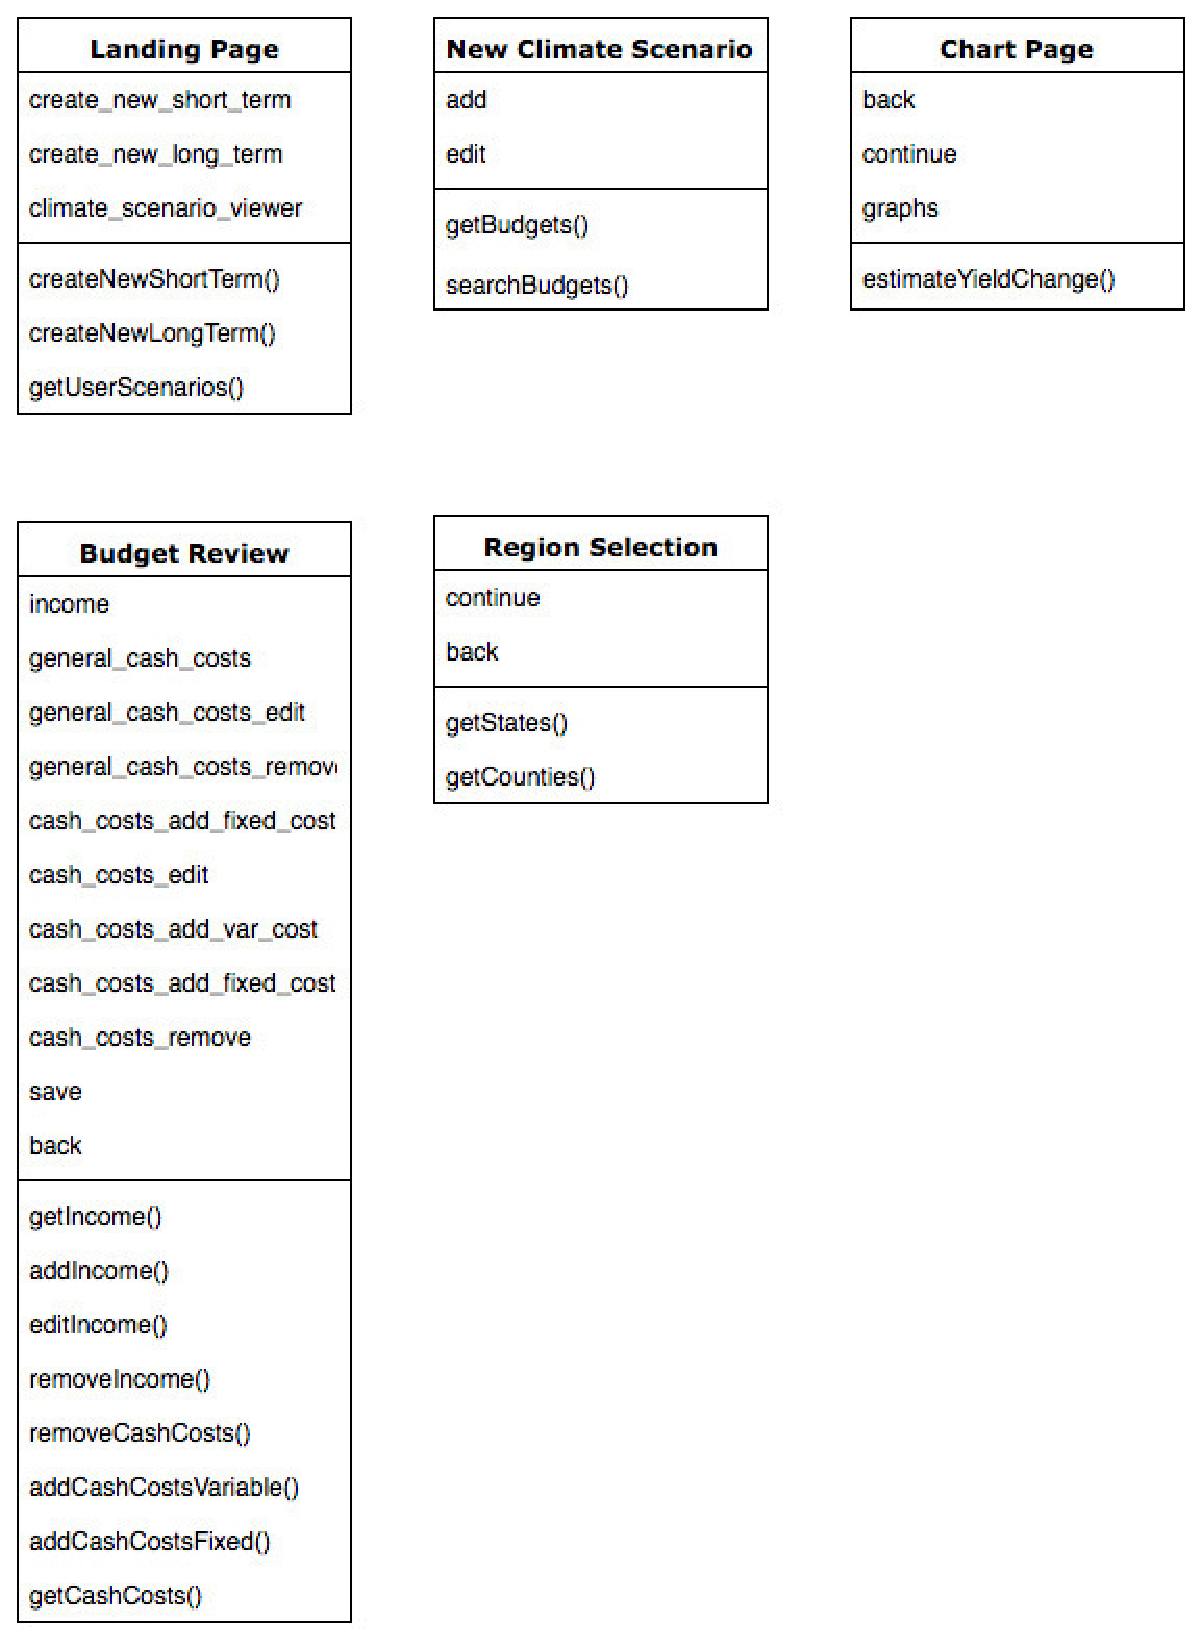
\includegraphics[width=300pt]{UMLDiagrams/angularComponents.eps}
		\end{center}
		\caption{Overall structure for Controller and View}
		\label{fig:Angular}
		\end{figure}
		
		\subsubsection{Landing Page}
		 The landing page has three angular components: create\_new\_short\_term, create\_new\_long\_term, and climate\_scenario\_viewer. The create\_new\_short\_term and create\_new\_long\_term are clickable action components that utuilize the createNewShortTerm() and createNewLongTerm() functions to make calls to the back-end and begin the climate creation scenario processes. The climate\_scenario\_viewer component  is used to make a call to the back-end using getUserScenarios() which grabs all scenarios tied to that user and presents them in a table.\\
		
		\subsubsection{New Climate Scenario}
		The new climate scenario page has two angular components: add, and edit. The add component allows users to add a new budget to their scenario from a list of provided budgets and the edit component allows users to alter budgets they already have attached to their accounts. There are two primary function calls associated to this page. The first function is getBudgets() which makes a call to the back-end to grab all available budgets for the user to select from. The second function is searchBudgets() which allows users to search for a specific budget from the list of all budgets.\\
		
		\subsubsection{Region Selection}
		 The region selection page has two angular components: back, and continue. These components are clickable and cause redirects to the previous new climate scenario page or the chart page. The two functions included in this page are getStates(), and getCounties() which make calls to the back-end to grab a list of all available states and counties that AgBizClimate has seasonal weather data for.\\
		
		\subsubsection{Chart Page}
		The chart page has three angular components: back, continue, and grab. Back, and continue clickable event buttons that are used to return to the previous page or move on to the next page. The graph component is a static component that displays the seasonal precipitation and temperature for the location they selected. This page also makes use of the function estimateYieldChange() which takes user input and makes a call to the back-end to use an AgBizLogic formula to make a more accurate budget review for the user.\\
		
		\subsubsection{Budget Review Page}
		The budget review page has the most angular components for viewing and manipulating data. There are also clickable navigation components back, and continue which allow users to go back to the previous chart page or continue on and save their current climate scenario. Next, there are a series of components that allows actions to be taken on the income and cash\_cost data objects. New income objects can be added via the income\_add component, edited via the income\_edit component, or removed from the list via the income\_remove component. cash\_costs can be edited via the cash\_costs\_edit component, assigned additional variable costs via the cash\_costs\_add\_var\_cost, assigned additional fixed costs via the cash\_costs\_add\_fixed\_cost component, or removed via the cash\_costs\_remove component. Finally, There are a series of functions that these components use to make calls to the back-end to retrieve and manipulate data. The getIncome() and getCashCosts() functions retrieve the income and cash\_costs associated with the budget to be displayed in the view. The addIncome(), addCashCostsFixed(), and addCashCostsVariable() functions are all used to add an aditional data object to the data objects or data object lists. The removeIncome() and removeCashCosts() functions are used to remove specific items from the list. Lastly, the editIncome(), and editCashCosts() functions are used to manipulate selected income and cast\_costs data objects.\\
		

	\subsection{Controller Design}
			\subsubsection{Overview}
			As an interface between Model and View, the Controller plays a very important role in the entire application architecture. First, it controls the way the application responds to the requests that result from the end-users' operations on UI. Secondly, it maintains the underlying relations between user interface (View) and data (Model). Thirdly, it accepts input from end-users, makes some necessary transformations, and then applies the final results on the data (Model). In this way, it controls the computation of the data (Models). At the same time, it could also reflect the variations on data (Model) back into UI (Views). \\
			\subsubsection{Overall Design}
			Overall, the controller tries to decompose the coupling between Model and View. However, as we would mainly employ the python Django framework for the whole AgBizClimate project. The Controller component acts as intermediary agent between front-end UI and back-end Climate APIs. However, it should be noted that the Django framework does not do well at separating the View and Controller clearly. As a result the view and controller are tightly interwoven. Therefore, it is better to deliberately define a middle layer between view and controllers. In this project, we could adapt some design pattern techniques called Mediator and Event dispatch mechanism. The figure \ref{fig:Con} depicts the overall structure for Controller and View. We can see that the user action is sent to Controller from View through a Mediator to Controller. And the final effects of Controller on View are sent back to View through Mediator. And the user actions are transferred by event dispatching mechanism. Therefore, the complex dependency relations between Controller and View are largely broken.\\

	\begin{figure}[htb]
		\begin{center}
			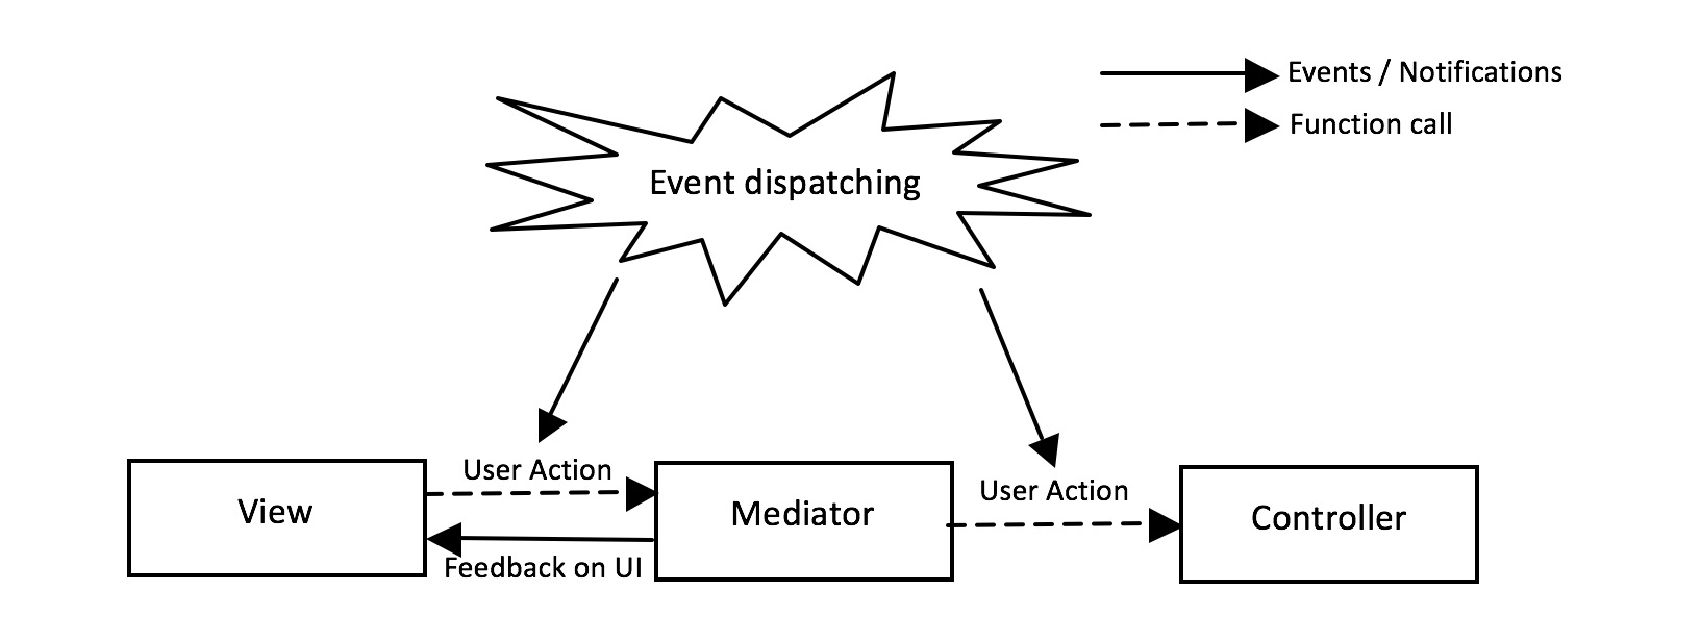
\includegraphics[width=300pt]{UMLDiagrams/Controller.eps}
		\end{center}
		\caption{Overall structure for Controller and View}
		\label{fig:Con}
		\end{figure}

		According to the data design, there are four kinds of general data types: user data, climate scenarios, budget data and the climate data. Consequently, we will need four general controllers to handle each data item. However, it is not possible or reasonable to deal with all of the business logic within the four general controllers. We plan to define some specific controllers to deal with more concrete tasks and organize them hierarchically. That is, underneath the four high level general controllers there are more low level small detailed controllers for various businesses / events. And the events are transferred gradually from lower levels to higher levels. In figure \ref{fig:TOPCon} presents the top Controller design of the AgBizClimate project. Basically there are two general controller types: Frontend Controller and Backend Controller, which mainly handles the operations/events from UI and data models, respectively. Additionally, much of the work are actually finished by the four specific controller under Backend Controller: Climate Scenario Controller, Climate Data Controller, Climate Factor Controller and Climate Budget Controller. Also, it should be noted that the Backend Controller will call the existing AgBiz Logic Model for certain tasks.\\

	\begin{figure}[htb]
		\begin{center}
			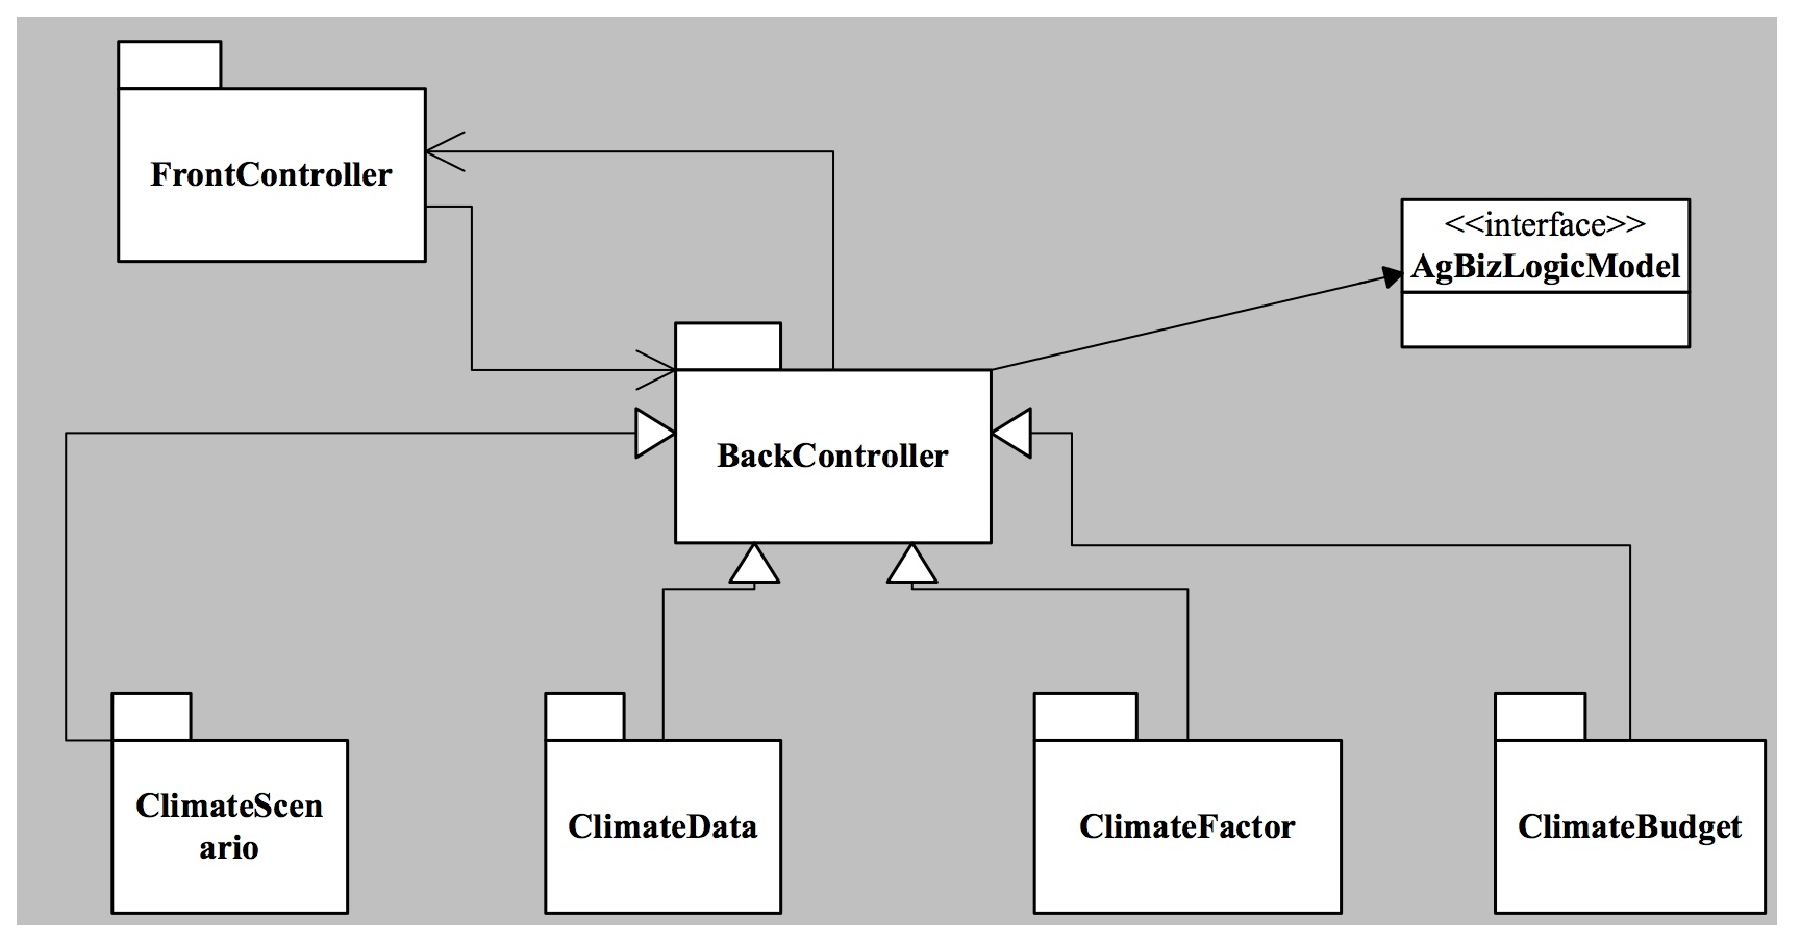
\includegraphics[width=300pt]{UMLDiagrams/TopController.eps}
		\end{center}
		\caption{Top controller design diagram}
		\label{fig:TOPCon}
	\end{figure}

	\subsection{API Design}
%here we will talk about the design of the API that will interface with the NWCTB.
		\subsubsection{Overview}
			In this section we will discuss the overall design of the API that will interface with the NWCTB. This API needs to get the data from the NWCTB, format the data, and send it to the client. Currently, there is a lot of uncertainty around the design of this API because we do not know what sort of API access that we will be given from the NWCTB. We are trying to contact the NWCTB development team regarding our API access but the NWCTB hasn't been very responsive. Because we still don't have NWCTB API access yet and have no date when this might be accomplished, we will discuss several possible options that do not require NWCTB API access along with one design option that includes NWCTB API access.\\

			\subsubsection{Diagrams}
				Shown below are two diagrams. The first diagram shows a UML design of this module shown in Figure \ref{fig:CDAPI}. Including the route for the API, the functions public and private and the data models used as part of this module. Also shown below in Figure \ref{fig:CDAPITrans} is how a typical transaction will work with the Climate Data API.\\
		\clearpage
		\begin{figure}[htb]
			\begin{center}
				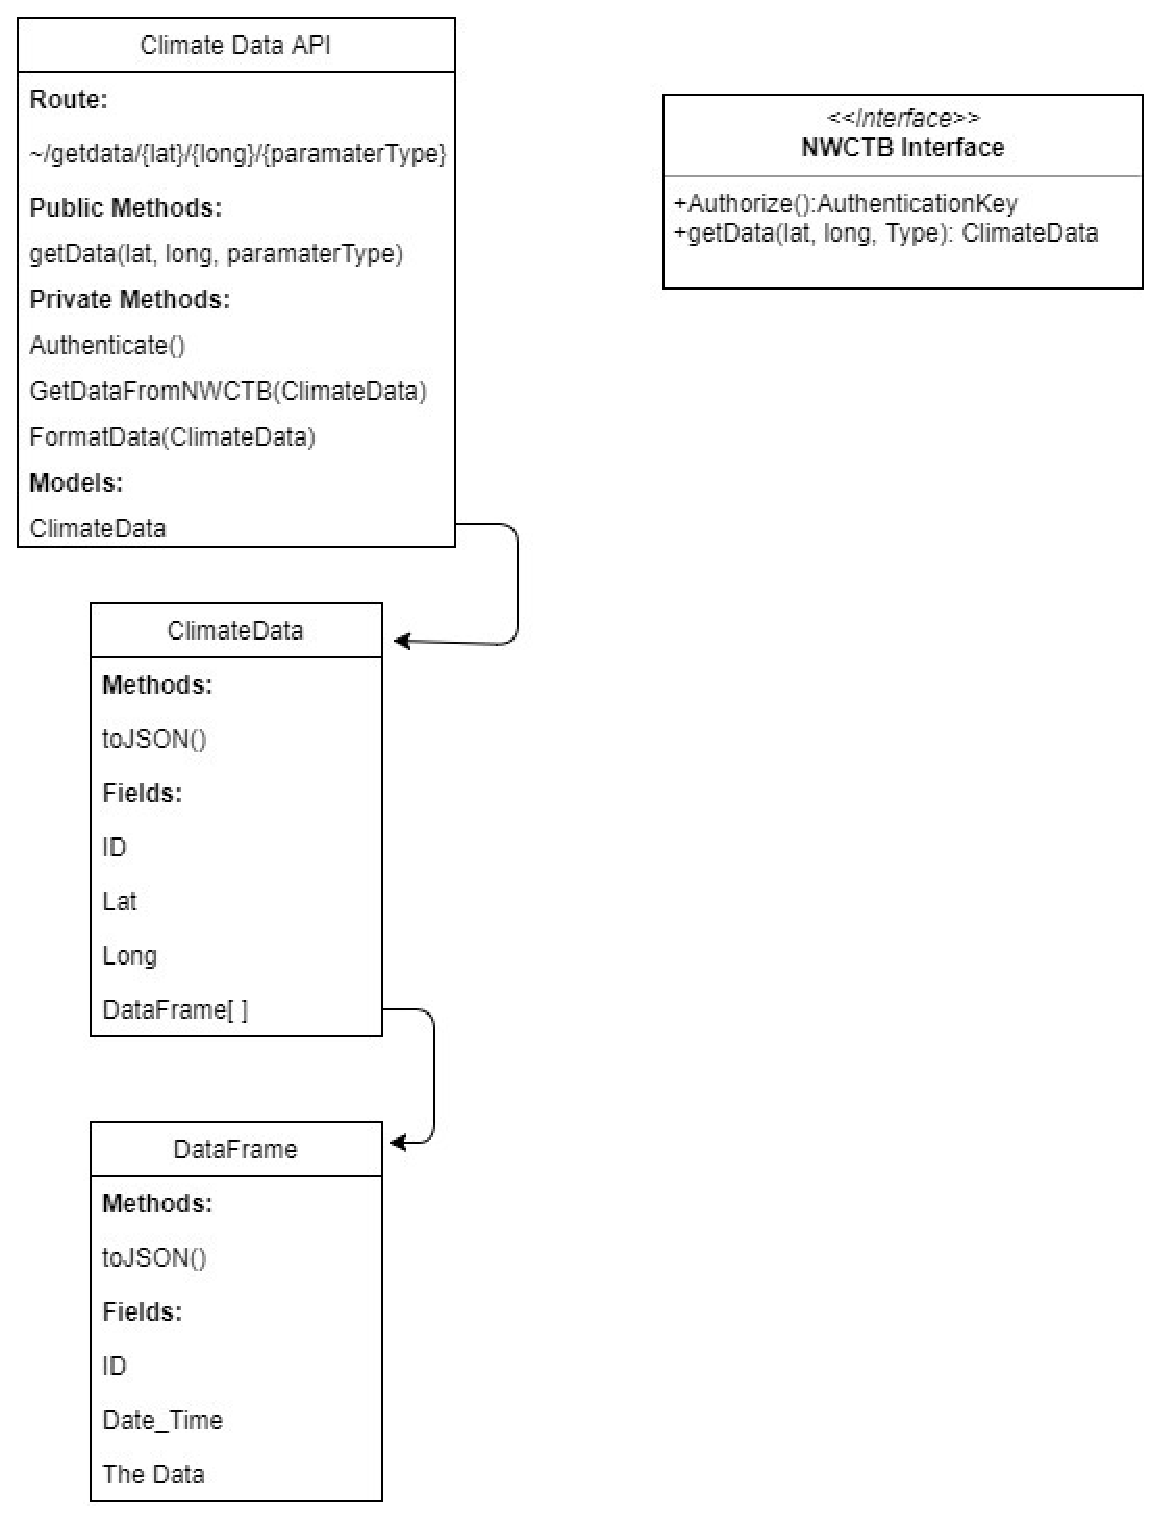
\includegraphics[width=375pt]{UMLDiagrams/ClimateAPI.eps}
			\end{center}
			\caption{Design of Climate Data API and associated models}
			\label{fig:CDAPI}
		\end{figure}
		\clearpage
		\begin{figure}[htb]
			\begin{center}
				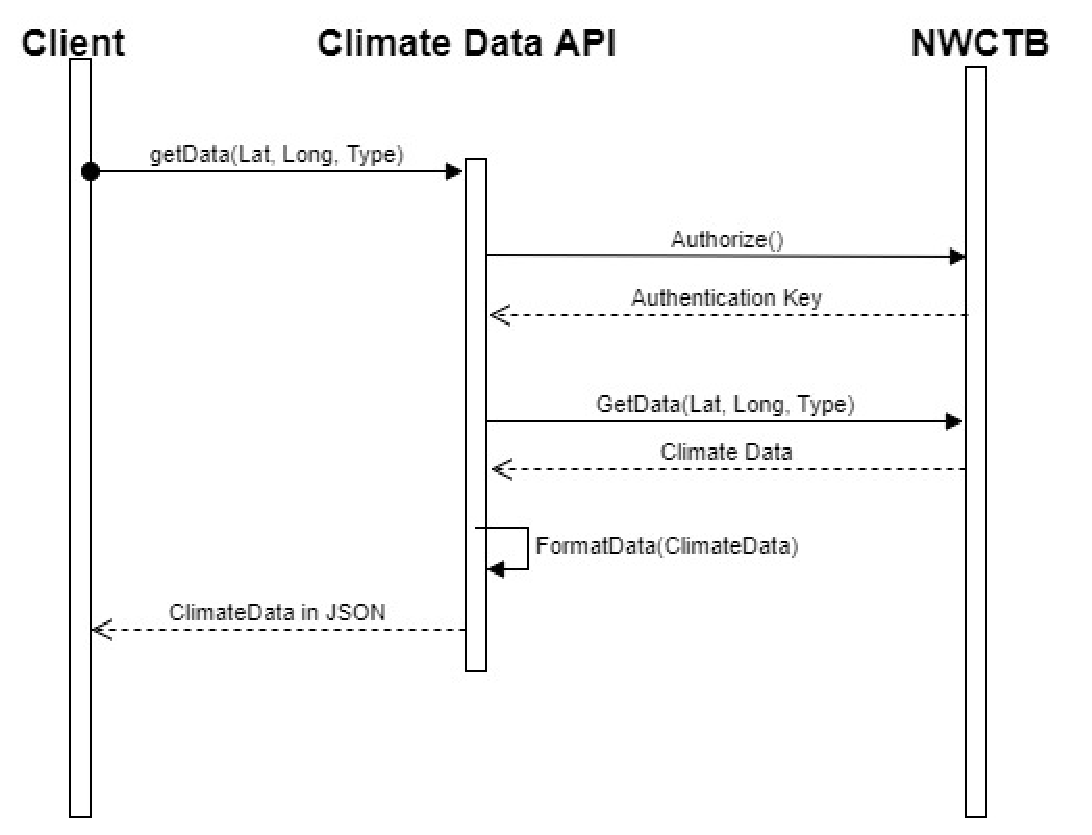
\includegraphics[width=300pt]{UMLDiagrams/ClimateDataAPITransaction.eps}
			\end{center}
			\caption{Typical Climate Data API Transaction}
			\label{fig:CDAPITrans}
		\end{figure}



			\subsubsection{Overall Design}
				The climate data API can be divided into three different parts. The API Controller it self, the Data that the controller will be using to represent the climate data and the NWCTB interface. The following paragraphs will briefly describe each of these components.
			\subsubsection{Function Design}
			In this section we will define and describe each function in the Climate API design. We will also discuss what each function will take as input and what each function will return.
					\paragraph{\textbf{Public Methods}}


					\paragraph{GetData(lat, long, parameterType)} - This function call takes three paramaters as input. latitude, longitude and parameter type. The parameter type is the type of data that the client is requesting either precipitation or temperature. This call will then return the requested climate data as a JSON object to the client.\\
					\paragraph{RouteCall: "~/getdata/\{lat\}/\{long\}/\{paramaterType\}"} - This route takes three parameters via the URL as input. These parameters are the latitude, longitude and the ParameterType. The parameter type is the type of data the user requested. In this case it's either precipitation or temperature. The data will then be formatted as a JSON object and will be returned to the calling client.\\

					\paragraph{\textbf{Private Methods}}

					\paragraph{Authenticate()} - This function will preform a hand shake with the NWCTB API to let the NWCTB API know who we are. This function will make a call to the Authorize function in the interface of the NWCTB API. This function will then get the authentication key for later use when we go to make requests to the NWCTB API.\\
					\paragraph{GetDataFromNWCTB(ClimateData)} - This function will set up and make the request to the NWCTB API. This function will take a ClimateData obejct as a parameter preloaded with the ID, Lat, and Long fields completed. This function will return the climateData object after initializing the DataFrame collection with the data received from the NWCTB.\\
					\paragraph{FormatData(ClimateData)} - This function will take a climate data object and will transform the object into a JSON object and return it.\\

				\subsubsection{Model Design}
					In this section we will define and discuss the models we plan to use in the Climate Data API. For each model we will define and describe each data member and function.\\



				\subsubsection{NWCTB Interface}
					We will not be talking about how the NWCTB Interface is designed as for the purposes of this project this is a black box that returns the climate data we requested. However we will discuss the method calls we plan to use for the NWCTB API.\\

					It should also be noted that this sections is what we are guessing the API Access should look like. Currently we are unsure how we will be accessing the API and what the calls will look like. But for the purposes of the design of this system we have taken our best guess and what it might look like.\\

					\paragraph{\textbf{Methods}}


					\paragraph{Authroize()} - This function takes no parameters and preforms a handshake between our application and the NWCTB application. This function call will return an authentication key that we can use later to make function calls to the NWCTB API.\\
					\paragraph{getData(lat, long, Type)} - This call takes latitude, longitude and the data type we are requesting. The data type in this case will either be precipitation or temperature. This function will then return the data we requested or an error if the request we made was unauthorized or was a bad request.\\


			\subsubsection{Data Design}
			In this section we will discuss the design of the models that we will use for the Climate Data API. For each model we will define and describe the fields and methods.\\

			\paragraph{\textbf{ClimateData}}
				This model represents the climate data for one whole climate simulation.\\
			\paragraph{\textbf{Fields}}
			ID - This is an ID that uniquely identifies this ClimateData object. This will be used to find specific model runs.
			Lat - This represents that latitude at which this climate situation is located.\\
			Long - This represents the longitude at which this climate situation is located.\\
			DataFrame[] - This is a collection of data frames that make up the climate data for this climate simulation.\\

			\paragraph{\textbf{Methods}}
			toJSON() - This method takes the ClimateData object and turns it into the equivalent JSON representation.\\

			\paragraph{\textbf{DataFrame}}
				This model represents one frame of data for a climate simulation. A data frame represents one moment in time in a climate simulation. A collection of these data frames make up a climate simulation.\\

			\paragraph{\textbf{Fields}}
			ID - This is a Unique identifier that will allow us to identify the order that the data frames need to go in.\\
			Date\_time - This is the date time that this data frame occurs on in time.\\
			The Data - This is a place holder for the data. We currently do not have API access to the NWCTB. As a result we are not sure how the data will be formatted. Once we have the data from the northwest climate tool box we will able replace this place holder with the actual data for each frame.\\

			\paragraph{\textbf{Methods}}
			ToJSON() - This produces the equivalent JSON representation of the data frame.\\


			\subsubsection{Possible Alternative to the NWCTB}
				In this section we will discuss other possible solutions for getting our climate data other than using the NWCTB. We are discussing this because it is possible that we may not get API access to the NWCTB or that we will get access after this project is completed. Because there is some uncertainty regarding the API access we have come up with a few different options if we are unable to get the necessary API Access.\\

				\paragraph{\textbf{Automate Downloading the Data}} \hfill \break
				One possible solution to getting the data without downloading the data is to write a script to download the data from the website. The data is available for download on their website and It wouldn't be too difficult to create a scrip that goes to their website and download the data. There are some potential issues we may run it using this approach. Firstly, they may throttle our speed if we try to download to many data entries at once or to often. This may happen many times as a person goes through climate scenarios for different crops. One way to over come this problem would be to cache the data in a database locally. This would allow us to only ever grab a data set for a location once. However, with this approach we would need to find a way to ensure that this data is the most updated data. This is the preferred alternative if we do not end up getting the NWCTB API access.\\
				\paragraph{\textbf{Build a New Service From the Ground Up}} \hfill \break
				Another possible solution would be to build a new service that went out to the NOAA got the different climate predictions and averaged together the result. The model data used by the NWCTB is public record available to the public for download. It would be possible to create a new service that did essentially the same thing as the NWCTB but without the user interface. There are a few nice things about this solution in that it would give us control over the data from start to finish and would allow us to make calls to an internal service rather than an external one. However, this would have serious impacts on our development time. This would also be a rather complex problem that would require a lot of research. Preferably we will not use this option.\\
				\paragraph{\textbf{Find A New Climate Data API}} \hfill \break
				Finally, Another solution would be to find a different API for the climate data we need. Currently we are unaware if another Climate Data API exists that would suite the needs of our application. However, if we were to find one that provided the data we need changing the design of our application to accommodate the new API probably wouldn't cause big issues. Assuming we can find another data source this approach would be ideal.\\






	%We may want to abandon this section.
	\subsection{Testing Design}
		%Here we will talk about how we plan to test this project.
		\subsubsection{Front End Testing}
		We plan to test the front end using a Angular testing framework. Using this testing frame work we will test that every possible user interaction produces some sort of UI action. Essentially the idea is that we ant to test that our UI is responsive for every possible UI action.\\
		
		\subsubsection{Controller testing}
		Controllers are the workhorse of MVC. And the tests of them would to some extent guarantee the correctness of the business logic of the application. Basically, most controllers either render a view or handle form submissions. Thus the test of controller should mainly focus on the concrete user operations or response but not the entire framework or functionalists of the application. And these tests would be done in the phase of unit test. Generally, each test for controller may consist of two steps. \\
		Firstly, one launches a request to the controller method to be tested. This is mainly done by user inputs from the view. In practice, the mocking actions from testing frameworks would replace human operations to do this.\\
		Secondly, one verifies that expected response is received or certain effect has taken place. This step could also be done easily by auto testing frameworks after one has define appropriate test cases.\\


		\subsubsection{API Testing}
		For the API we will provide testing for every possible API route. We will also test that erogenous resumes result in correct response. Beyond that we will also test each function in the API. For each function we will test a variety of different inputs for each function including valid and invalid inputs. We will then ensure that the correct result is returned for valid requests. For invalid request we will ensure that the correct error message is returned.\\

%Here we will talk about the UI.
\section{User Interface Design}

	\subsection{Overview of User Interface}
	The user interface is an essential part of any web application as it is the layer between the user and what they want and need out of an application. In this section we will be discussing the User Interface. Specifically, we will be detailing the specific UI elements that make up each page.
	%I've already created screen images as part of another project. We should use those here. They are in the figures folder in the project.
	\subsection{Screen Images}
		\begin{figure}[htb]
		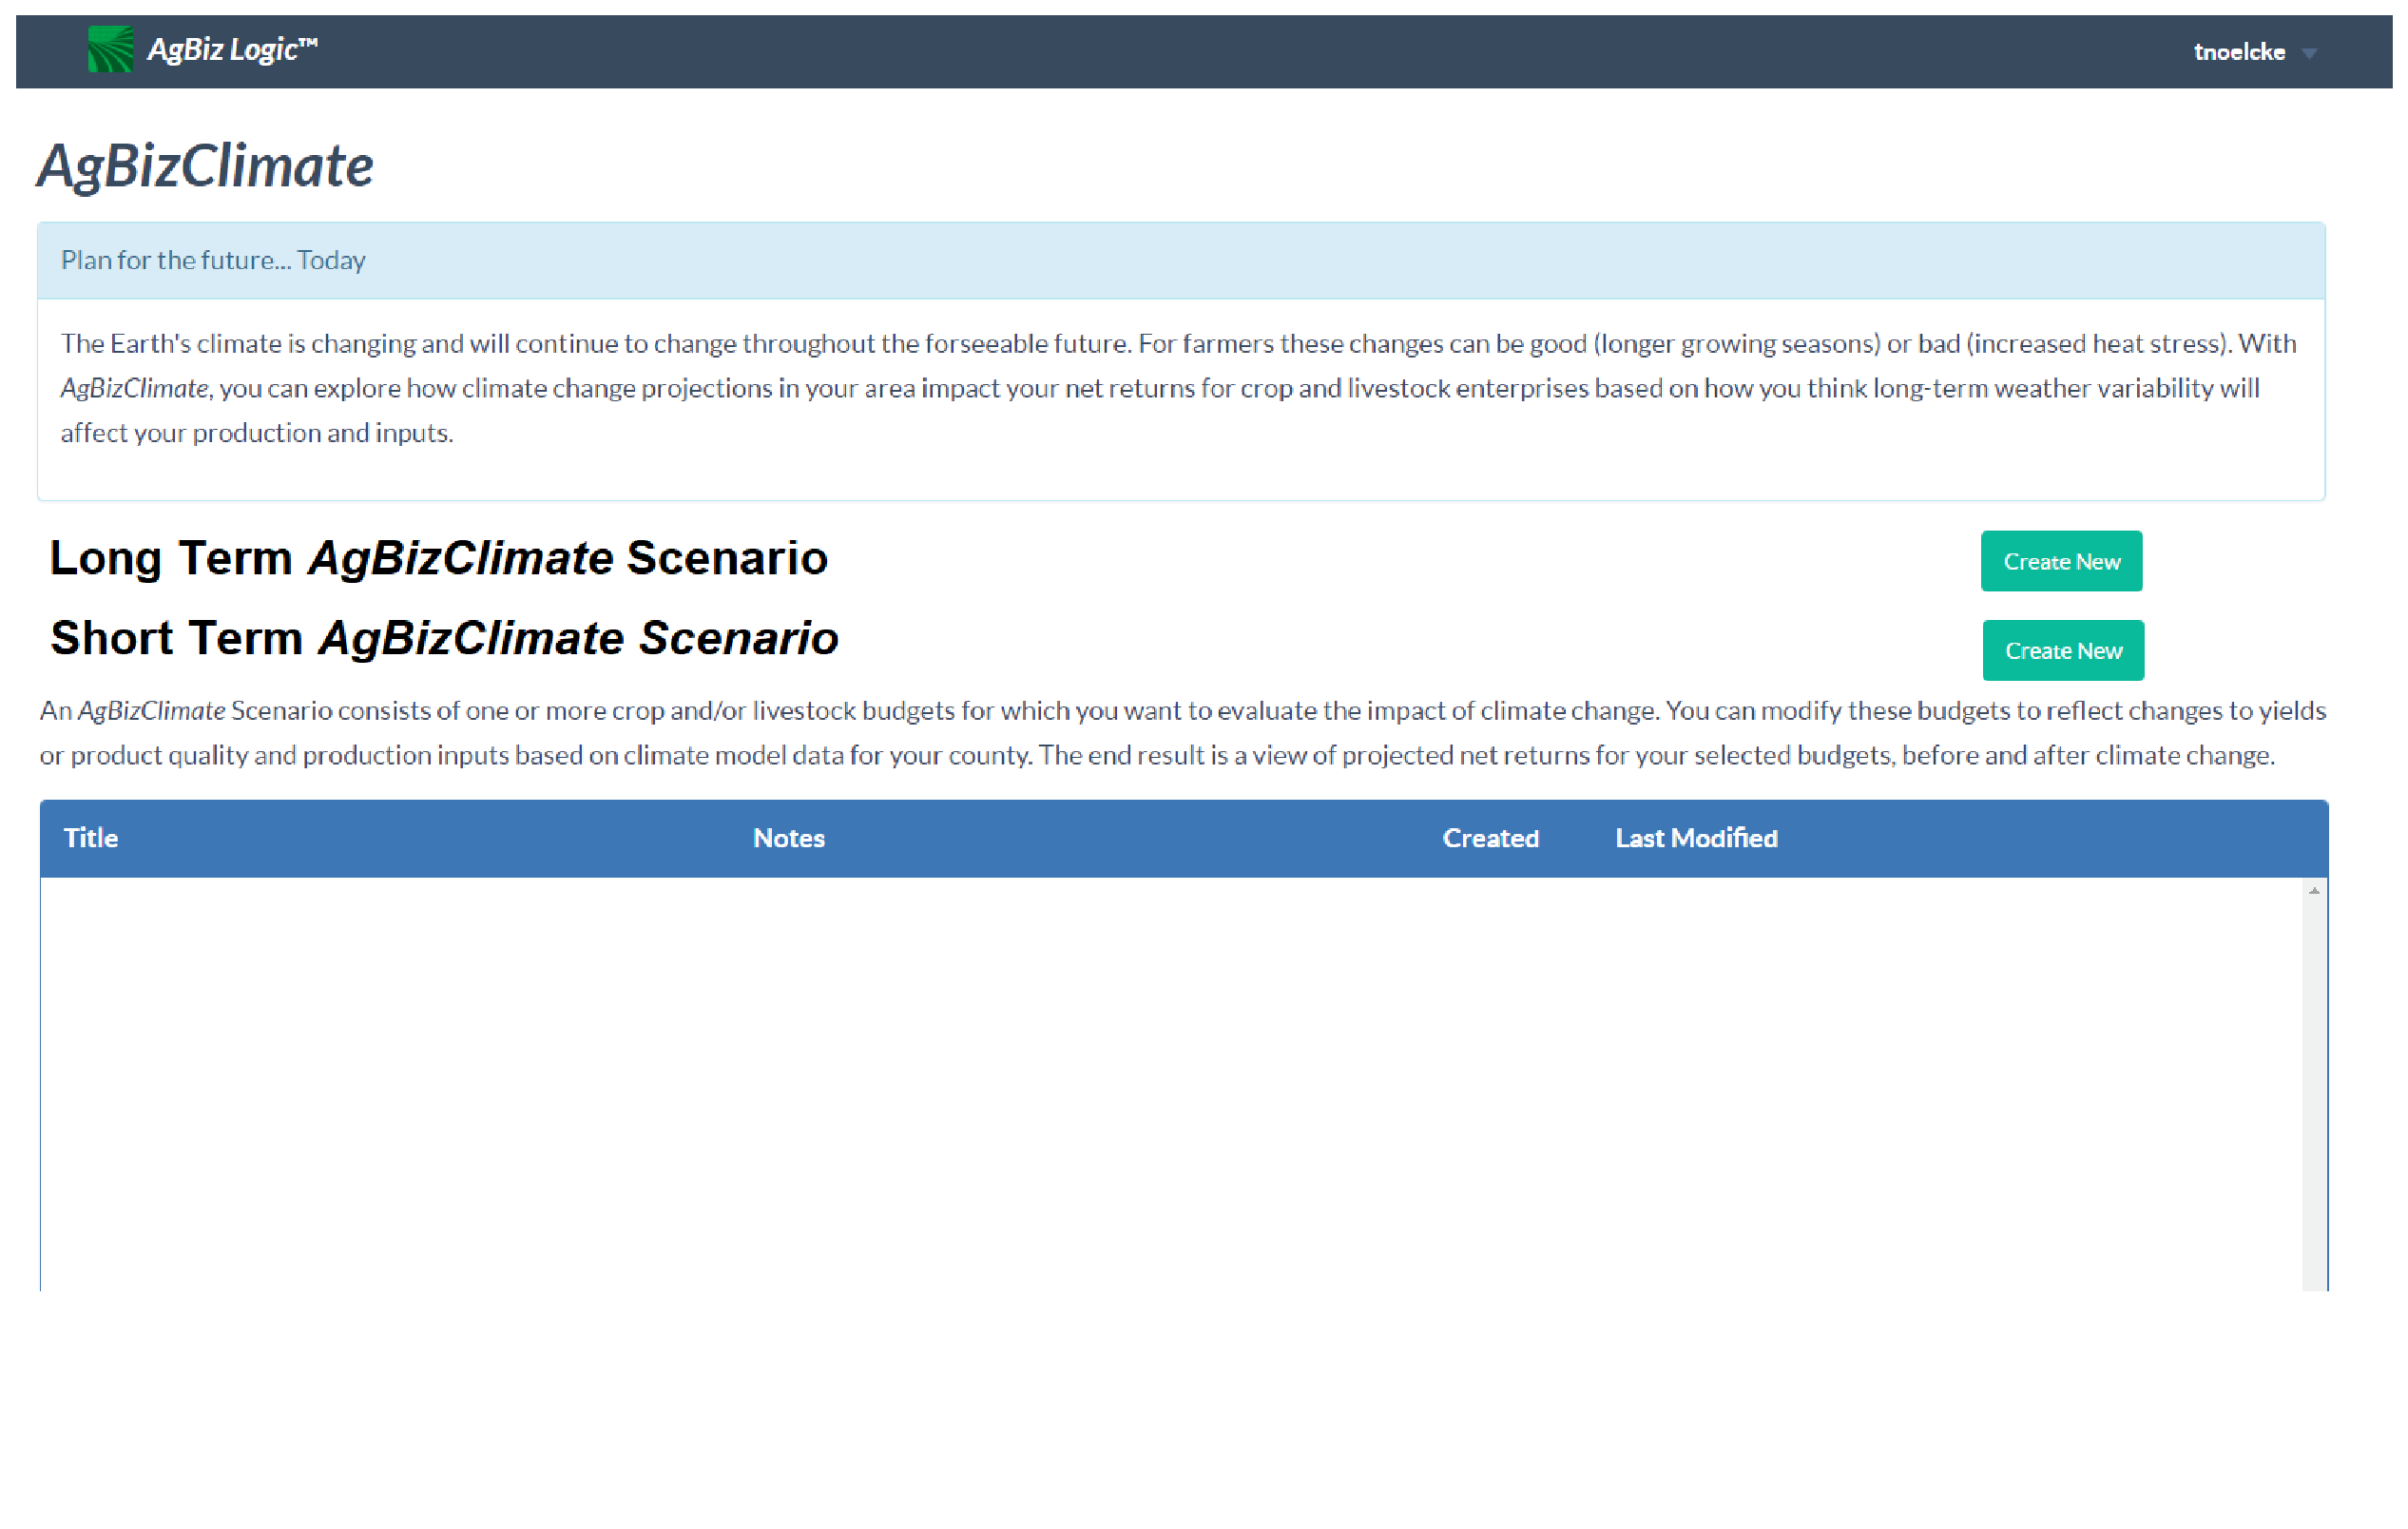
\includegraphics[width=\linewidth]{Figures/LandingPage.eps}
		\caption{Landing Page}
		\label{figure3.1}
	\end{figure}
					
	\clearpage
	\begin{figure}[htb]				
		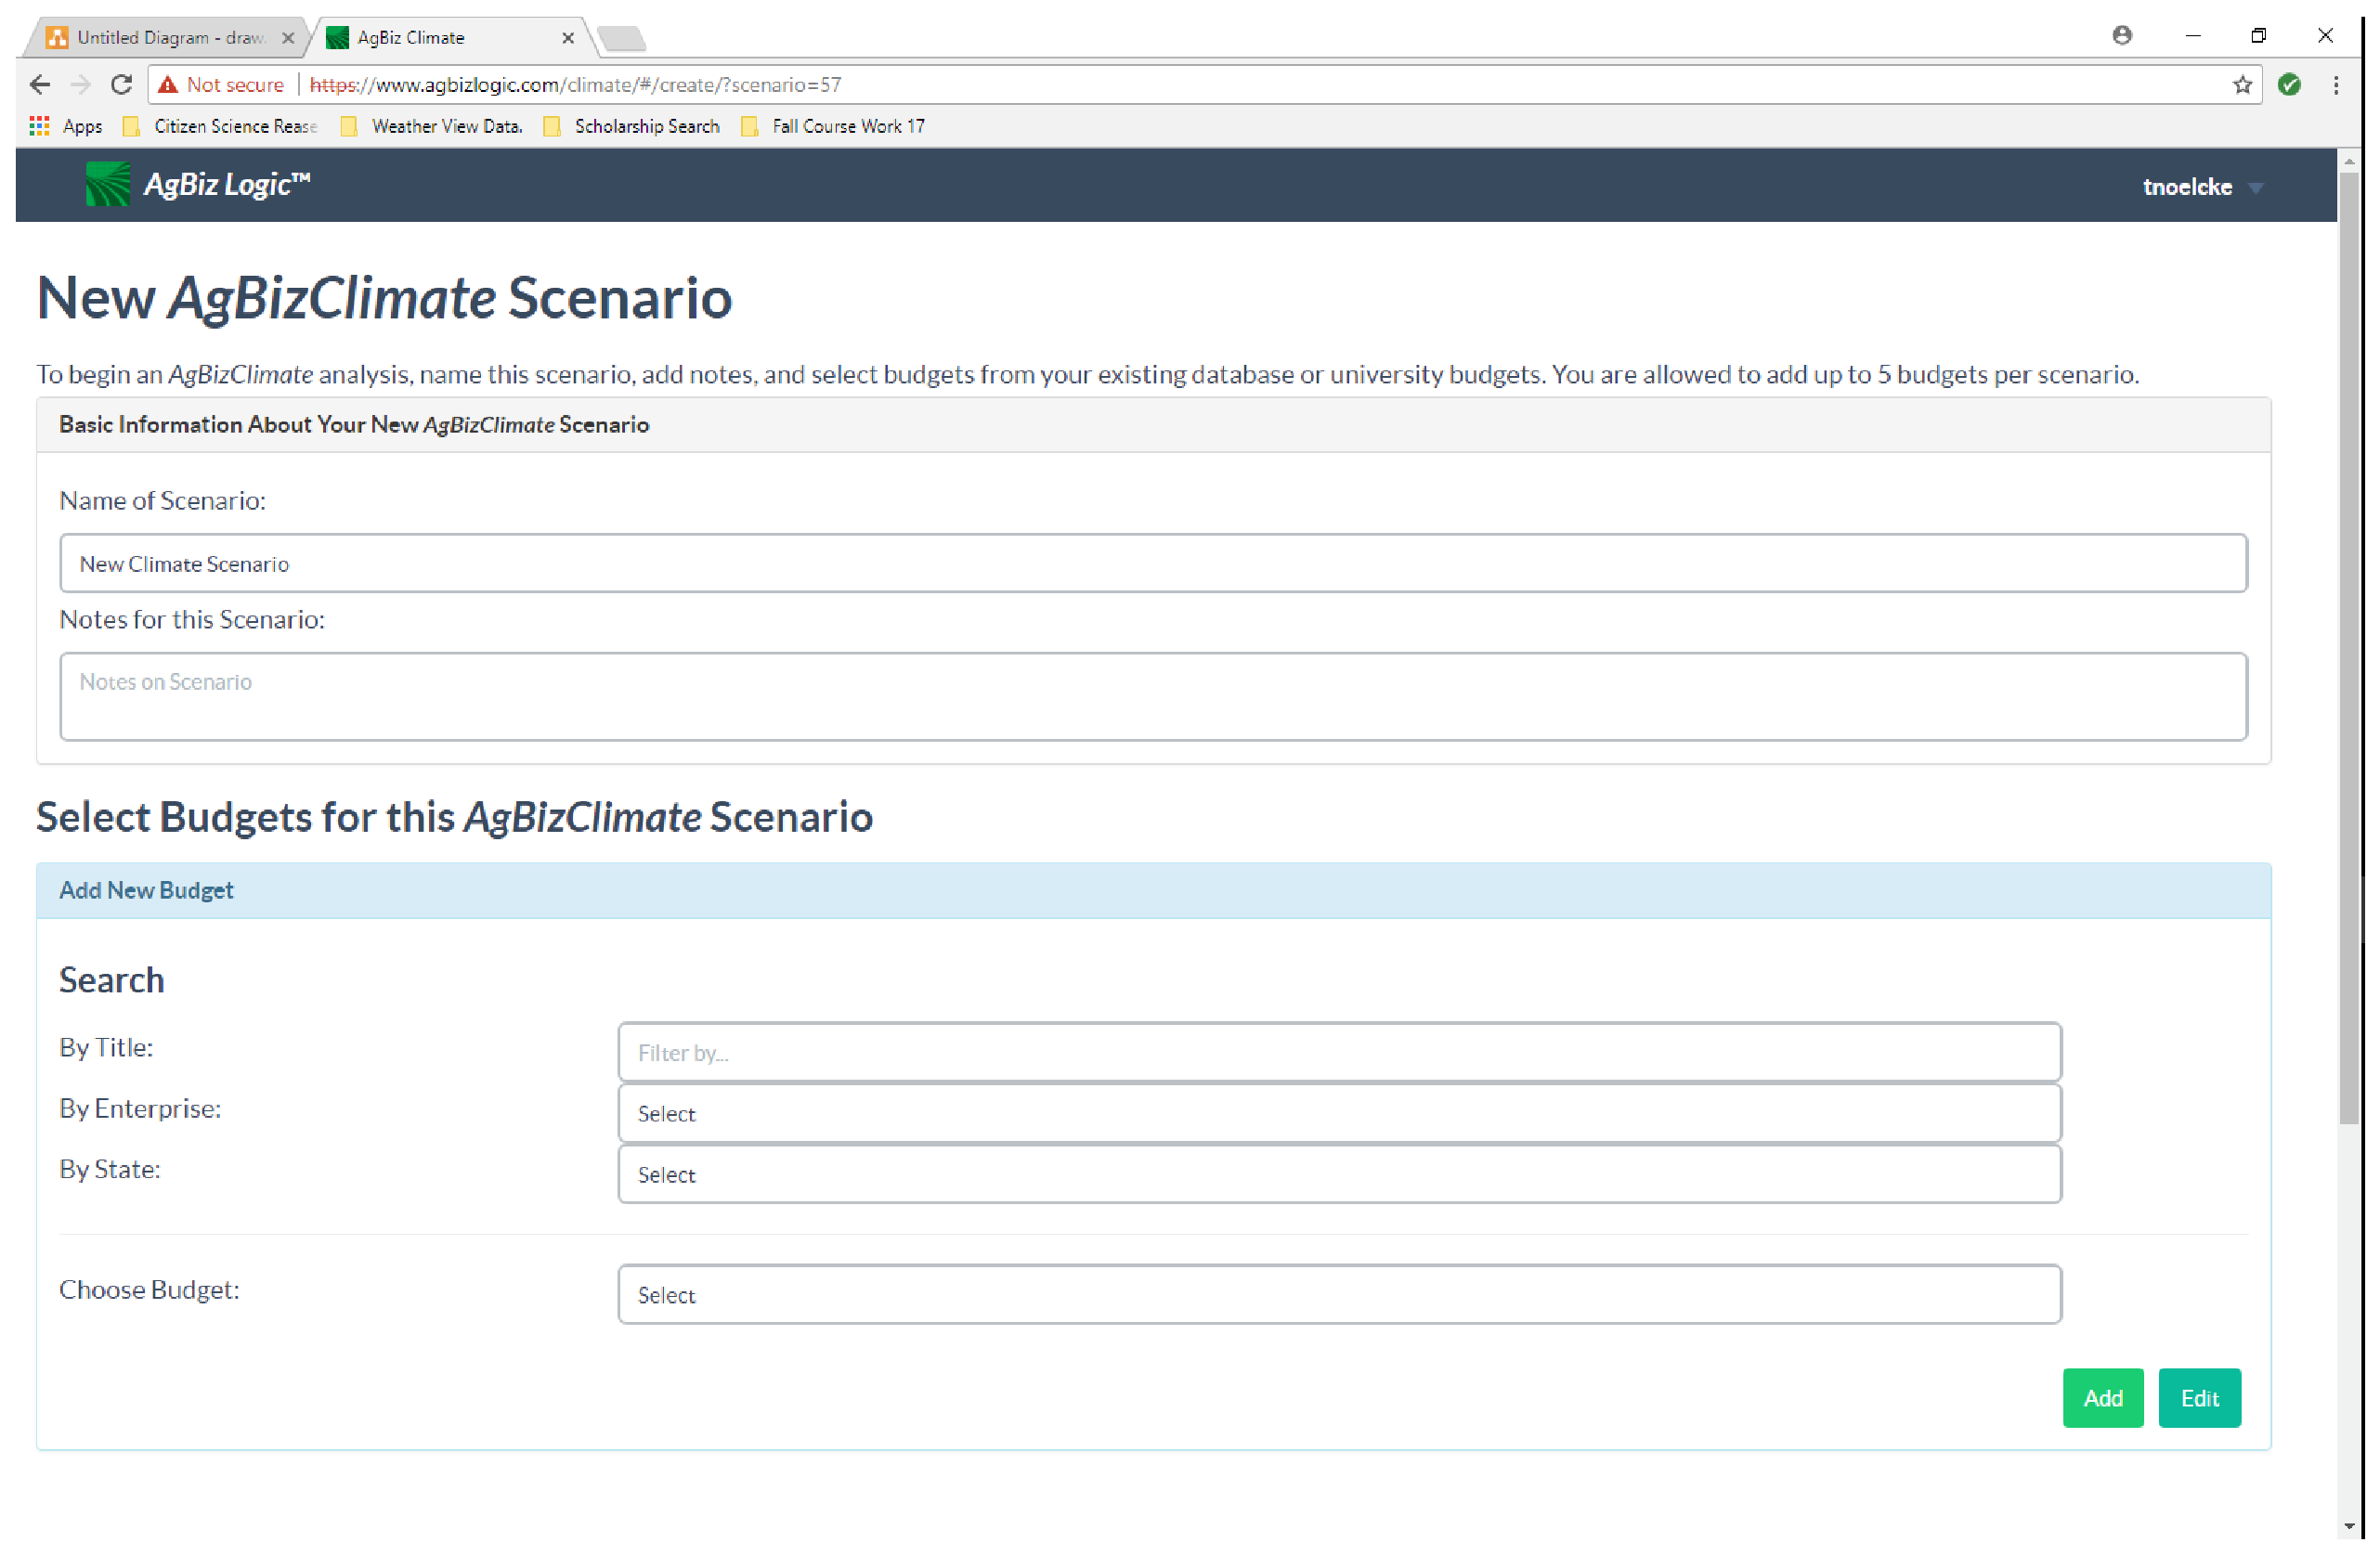
\includegraphics[width=\linewidth]{Figures/ClimateScenario.eps}
		\caption{Allows user to select budgets and make notes}
		\label{figure3.2}					
	\end{figure}
					
	\clearpage
	\begin{figure}[htb]
		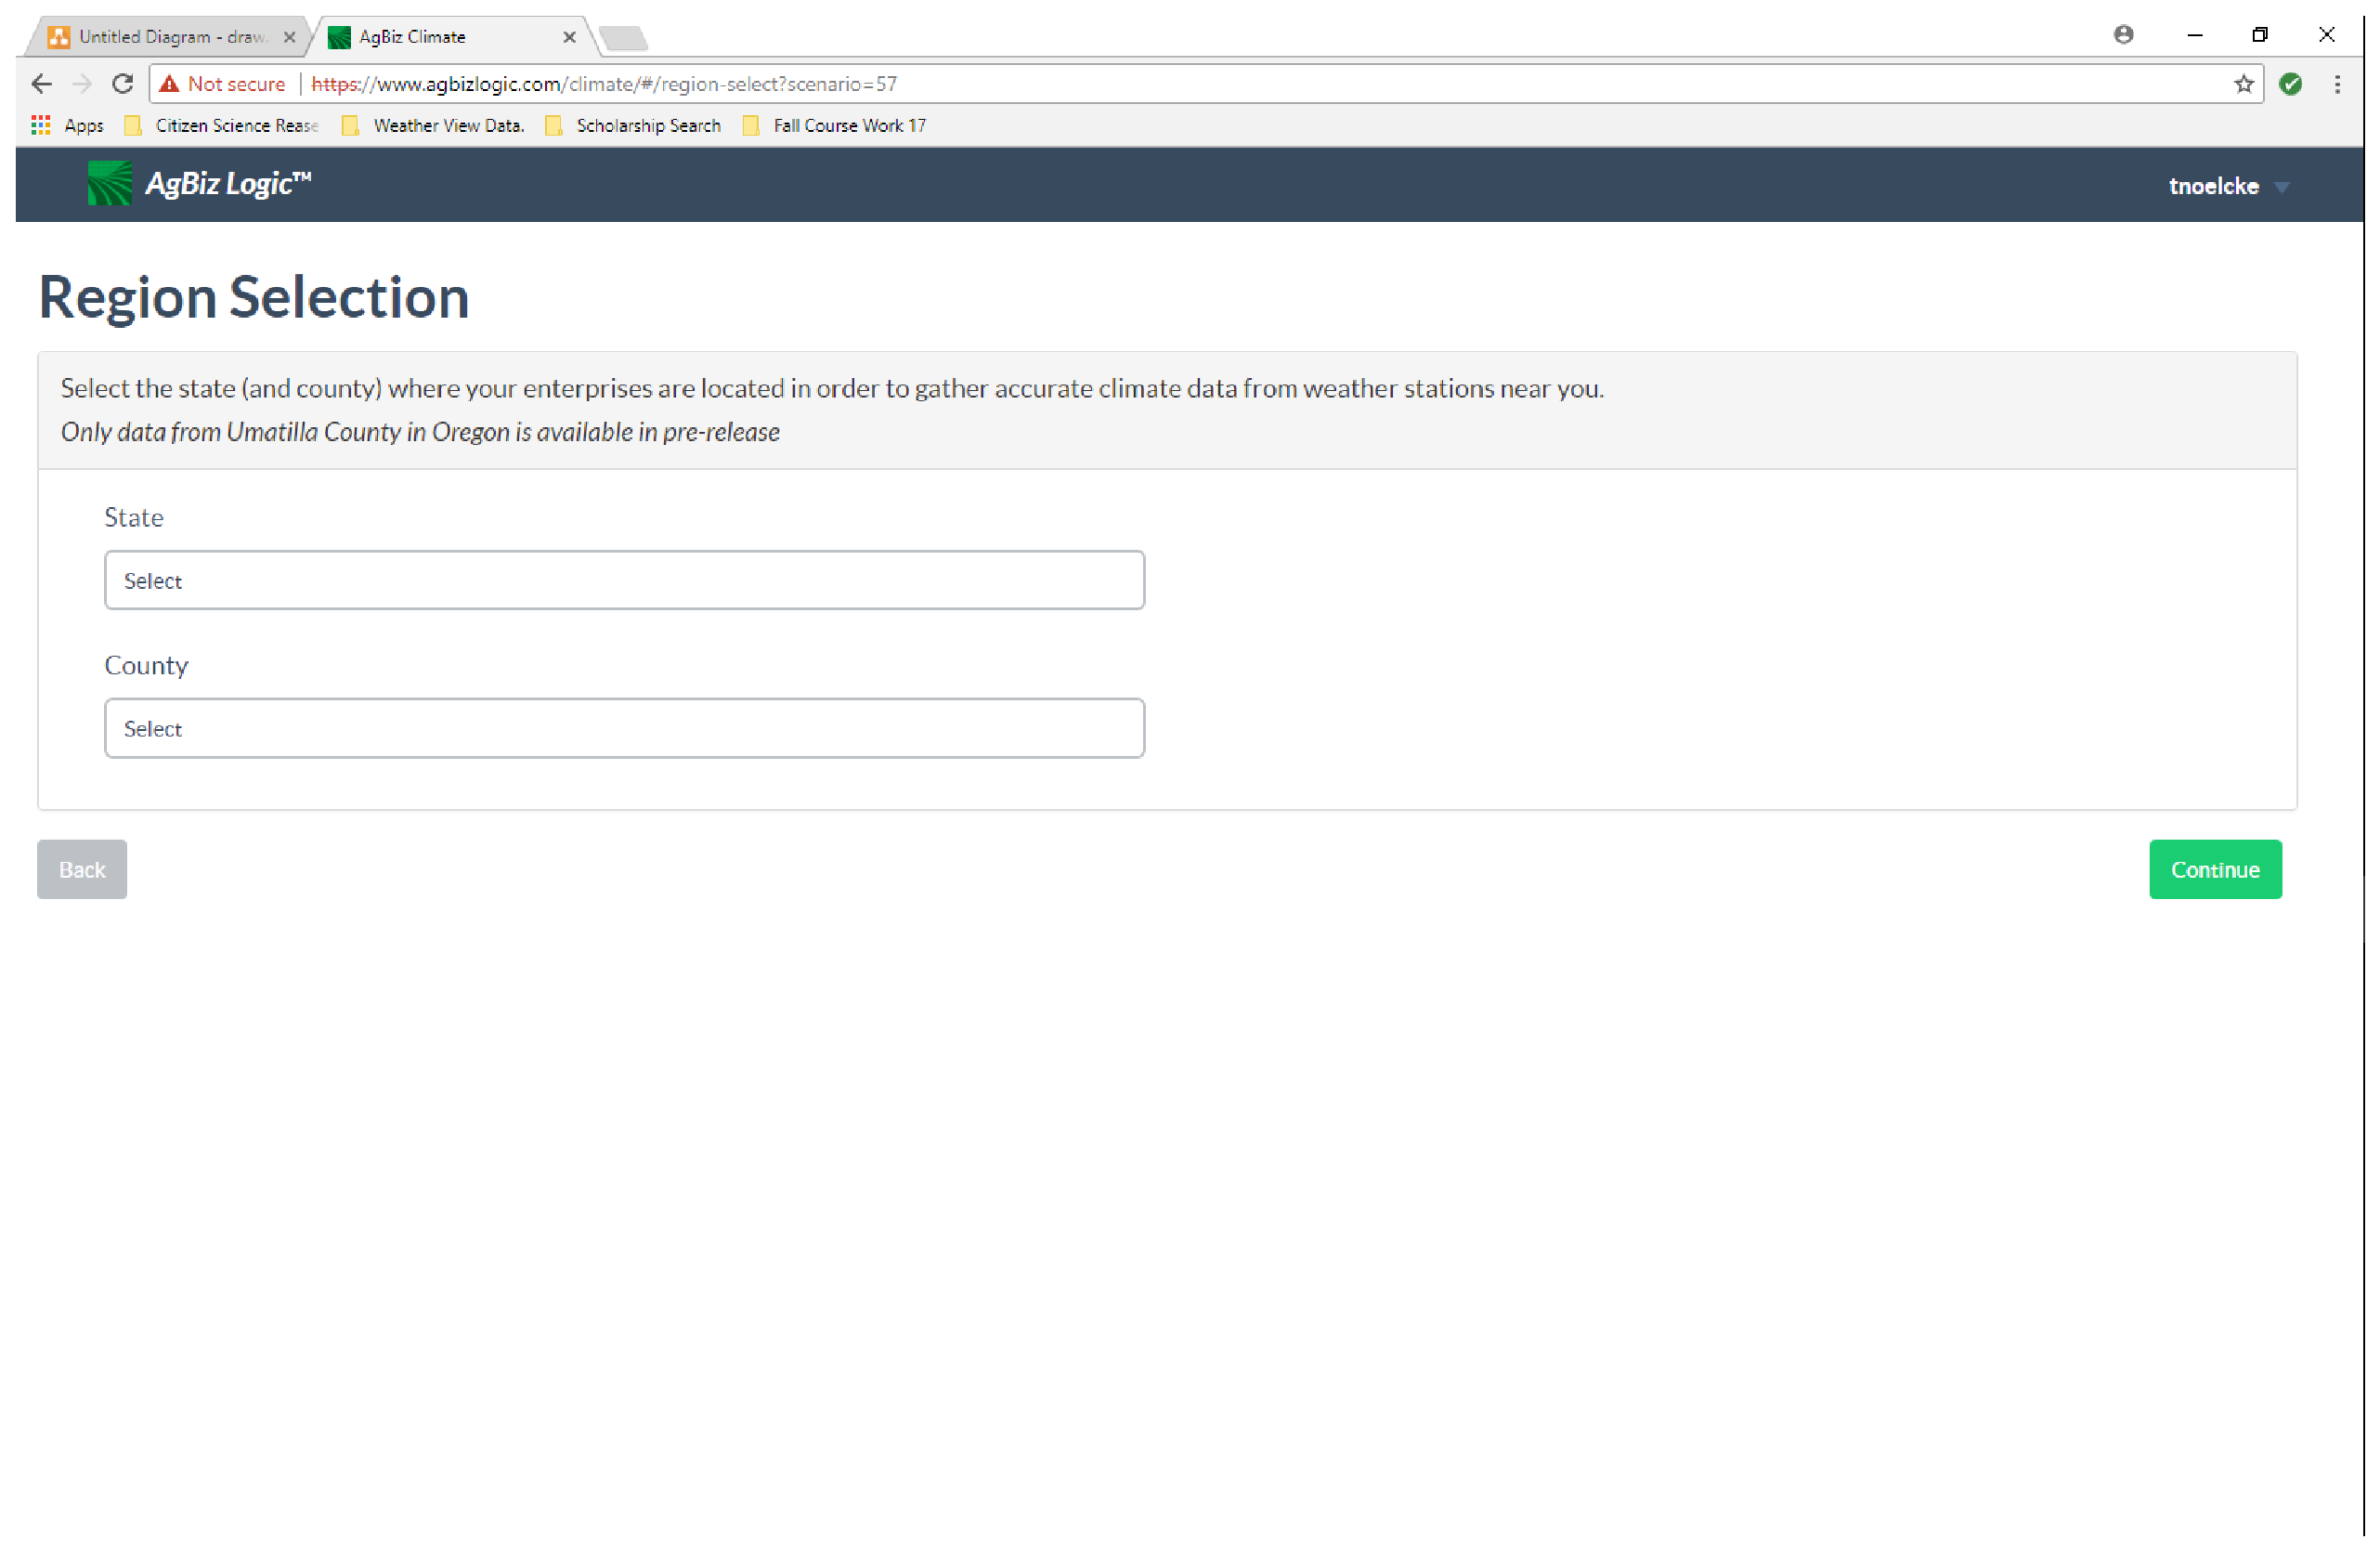
\includegraphics[width=\linewidth]{Figures/SelectStateAndCounty.eps}
		\caption{Allows User to select location}
		\label{figure3.3}
	\end{figure}
	
	\clearpage
	\begin{figure}[htb]
		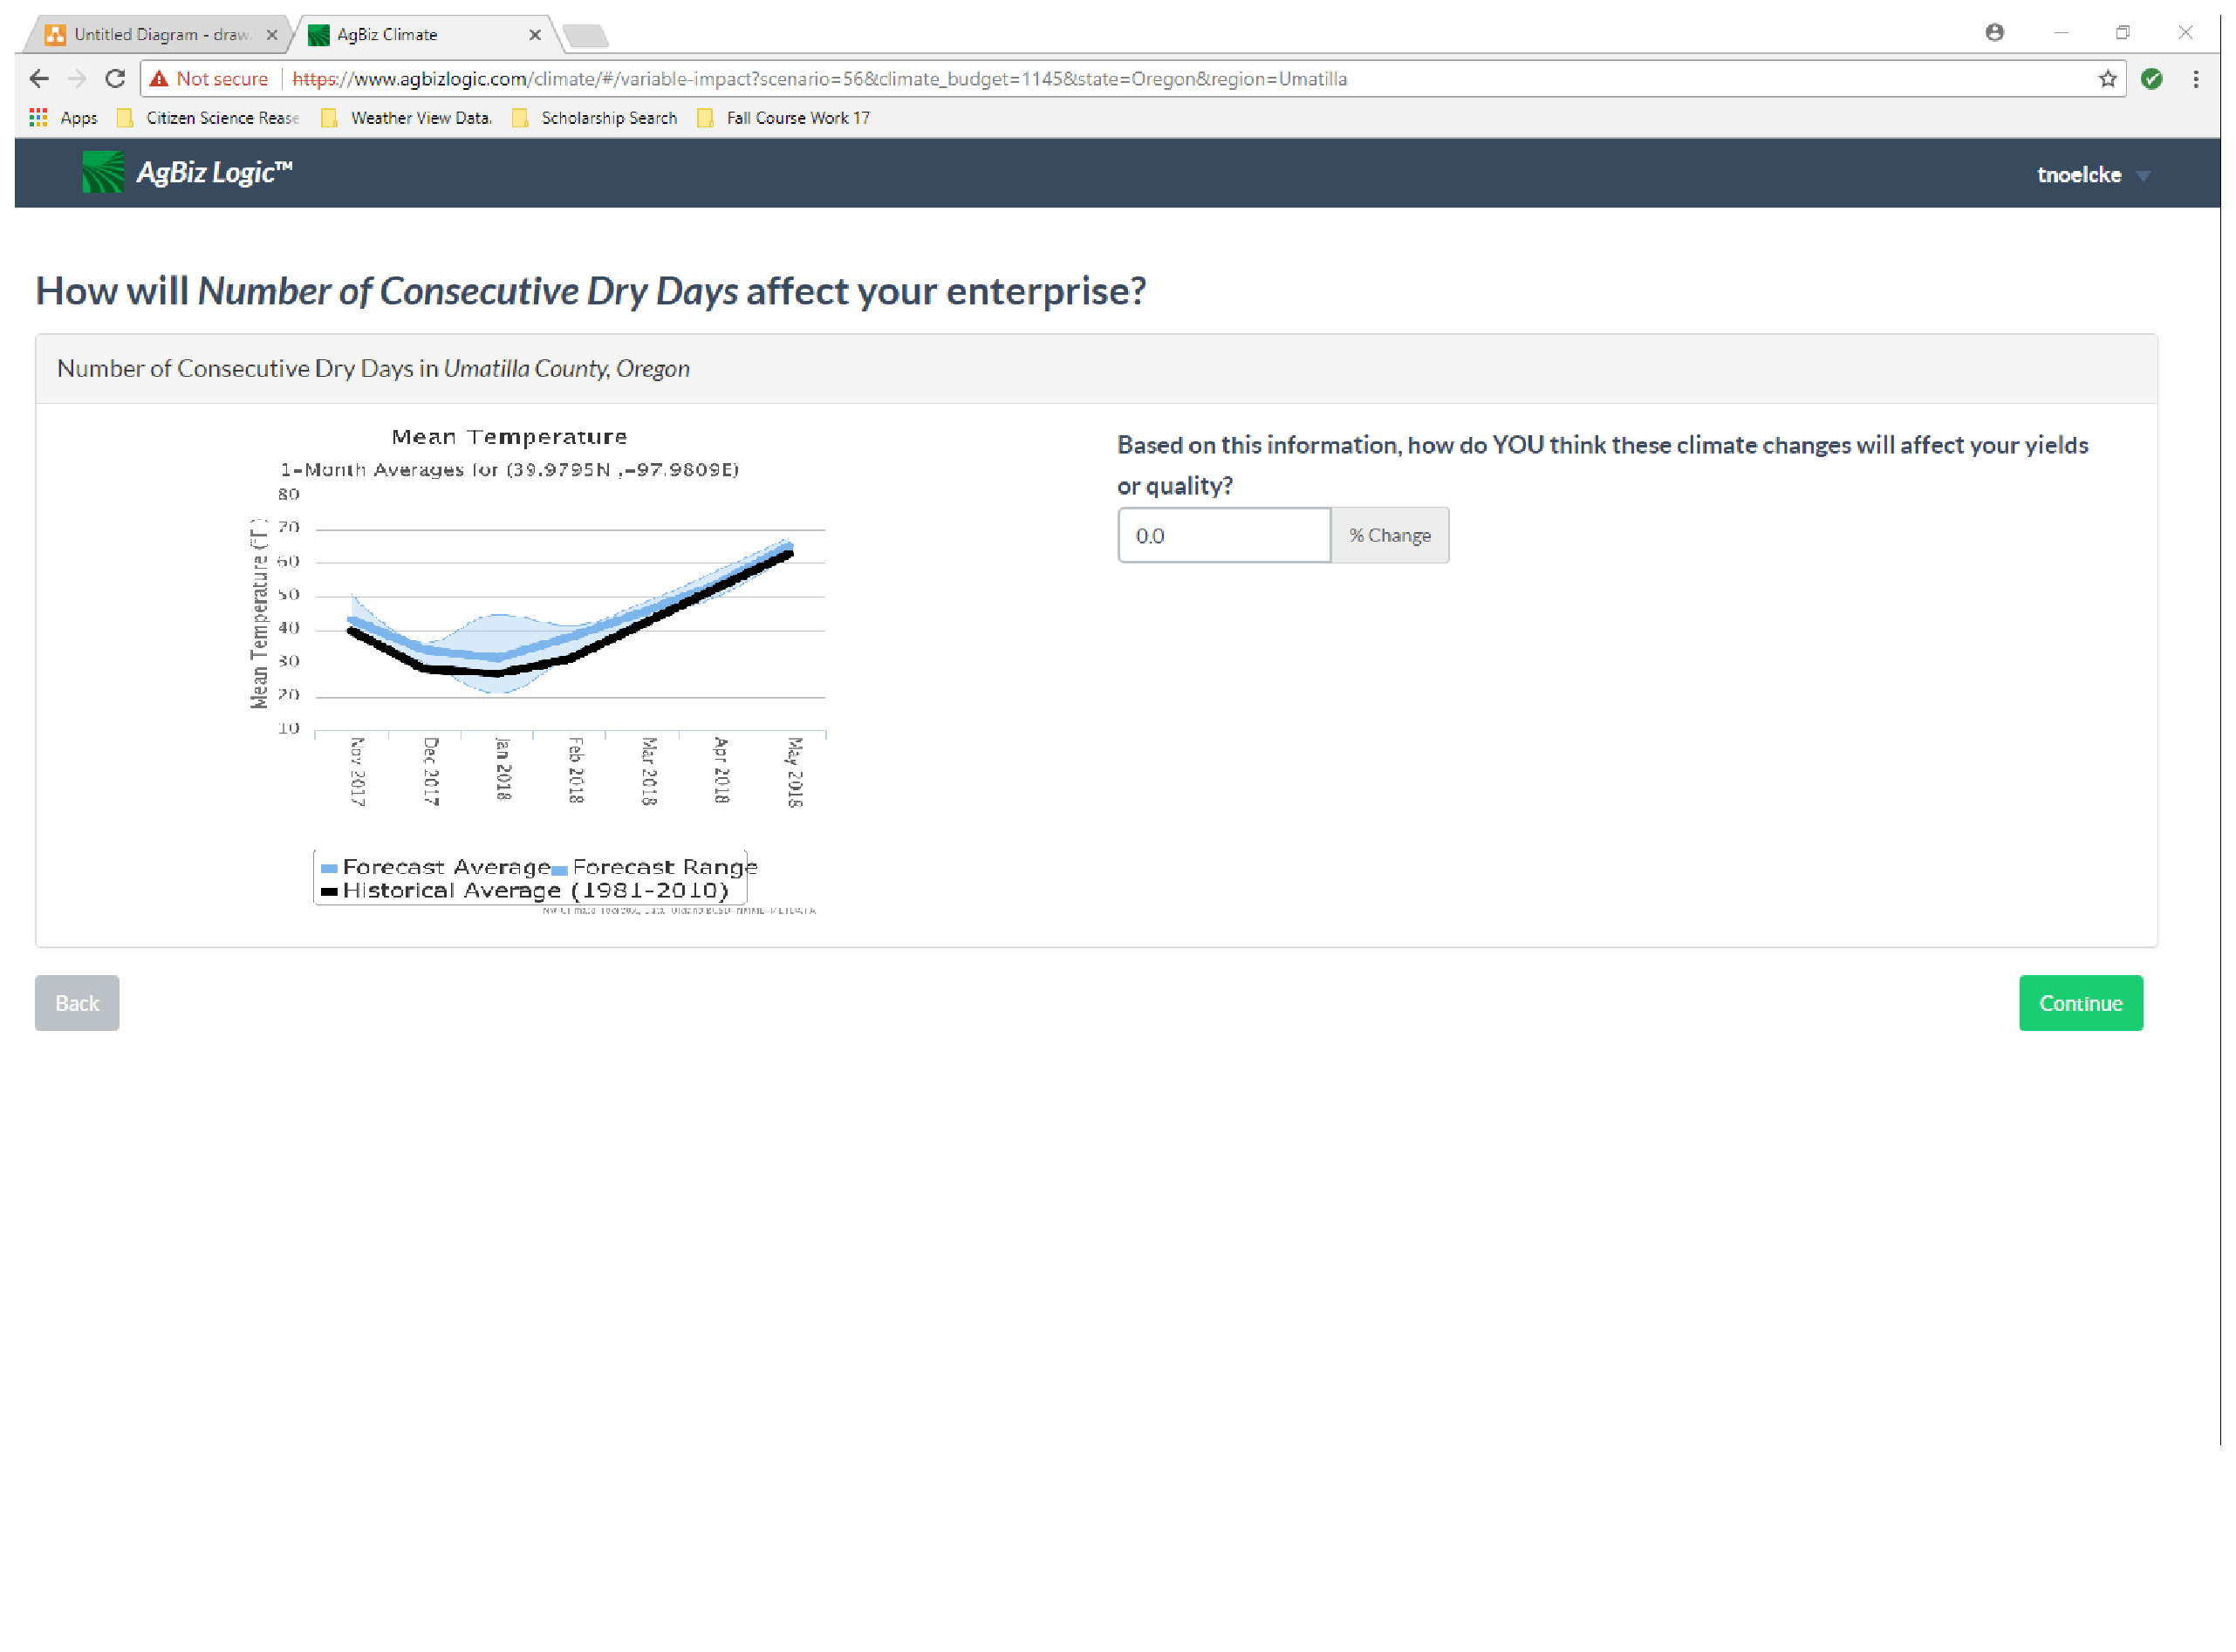
\includegraphics[width=\linewidth]{Figures/ChartPage.eps}
		\caption{Displays the Data in a plot}
		\label{figure3.4}
	\end{figure}
	
	\clearpage
	\begin{figure}[htb]
		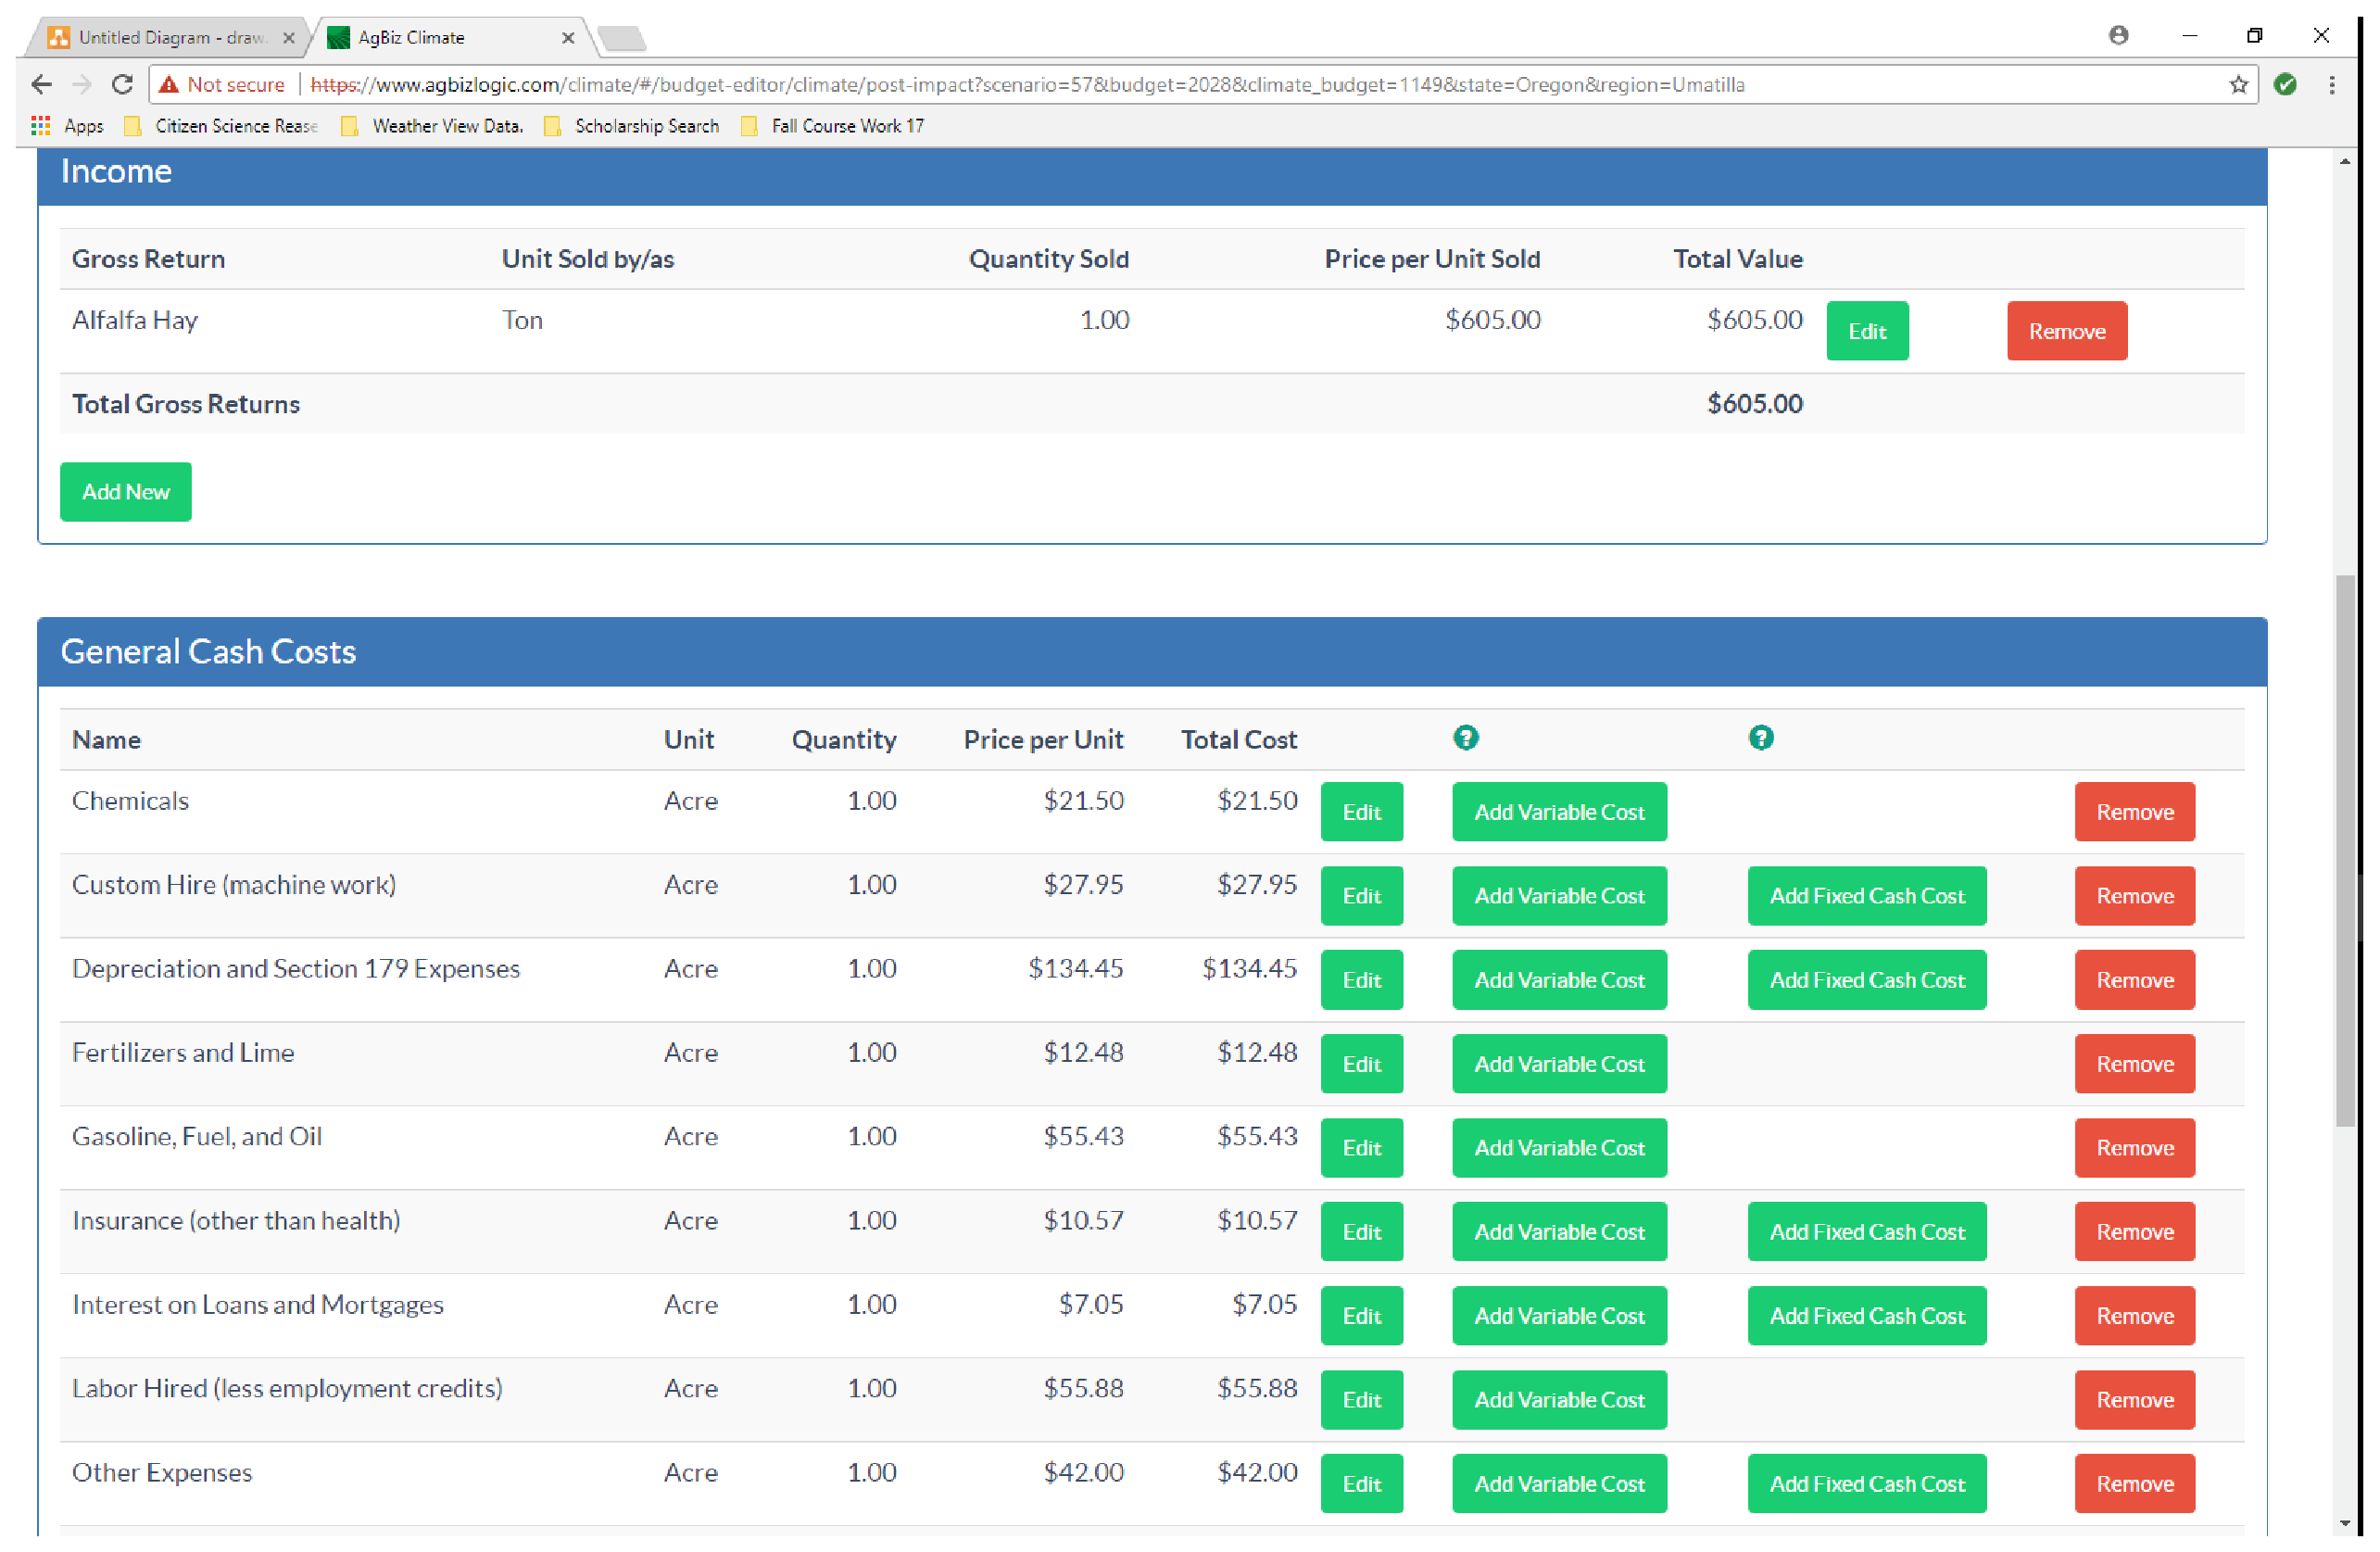
\includegraphics[width=\linewidth]{Figures/BudgetReivew.eps}
		\caption{Allows user to view their budget}
		\label{figure3.5}
	\end{figure}
	\subsection{Screen Objects and Actions}
		\subsubsection{Landing Page}
		The Landing page consists of two primary parts: the information jumbotron, new scenario creation, and a scenario listings. The information jumbotron is a static and gives the mission statement of the AgBizClimate product. The new scenario creation selection allows the user to click on one of two boxes specifying if they would like to create a new short or long term climate scenario. Finally, the scenario listings section is a dynamic table that provides information on the title, notes, date created, and date last modified for all entered climate scenarios.\\
		\subsubsection{Climate Scenarios}
		The new climate scenario page consists of three primary parts: the information section, and budget selection. The information section will state that the user is beginning a new AgBizClimate scenario and provide rules and data entry components for the scenario and notes for the new scenario. Specifically it will allow users to enter text specifying the scenario name and notes for the new scenario. Finally budget selection portion will allow users to add a budget or select a preexisting budget from the existing database.
		\subsubsection{Region Selection}
		The region selection page will consist of a jumbotron stating that the user is on the region selection page, a brief message explaining what the page is for, and two drop down boxes that the user can use to select the desired state and county for their new climate scenario. This page will also have a back, and continue button that allow users to either backtrack through the new climate creation process or move on to the new step.
		\subsubsection{Chart Page}
		The chart page will consist of a title prompting the user to consider how the following graph will affect their enterprise, a graph containing localized temperature, and precipitation data based on previous user input in the region selection page and a text box where the user can enter the percent they think the forecast will affect their yields or quality. This page will also contain the back, and continue buttons the other pages have which allow the user to more easily move around the tool. 
		\subsubsection{Budget Review}
		The budget review page will have two major section. The first section is the income section which is a table containing the following information: income gross returns, unit sold as, quantity sold, price per unit, and total value. This table will also sum the total value from this section for the user. The second section is a general cash costs section and contains the the following information: name, unit, quantity, price per unit, and total cost. Finally for each table users will have access to buttons that will allow them to add new entries, remove entries, and edit entries. 


\clearpage
%in this section we will show how are design will fufill the functional requirements.
\section{Requirements Matrix}
	Shown below in figure \ref{fig:ReqMat} is our requirements matrix. This matrix shows how the different components will fufill the project requirements. For a full list of requirements please see the AgBizClimate requirements document.\\


		\begin{figure}[htb]
			\begin{center}
				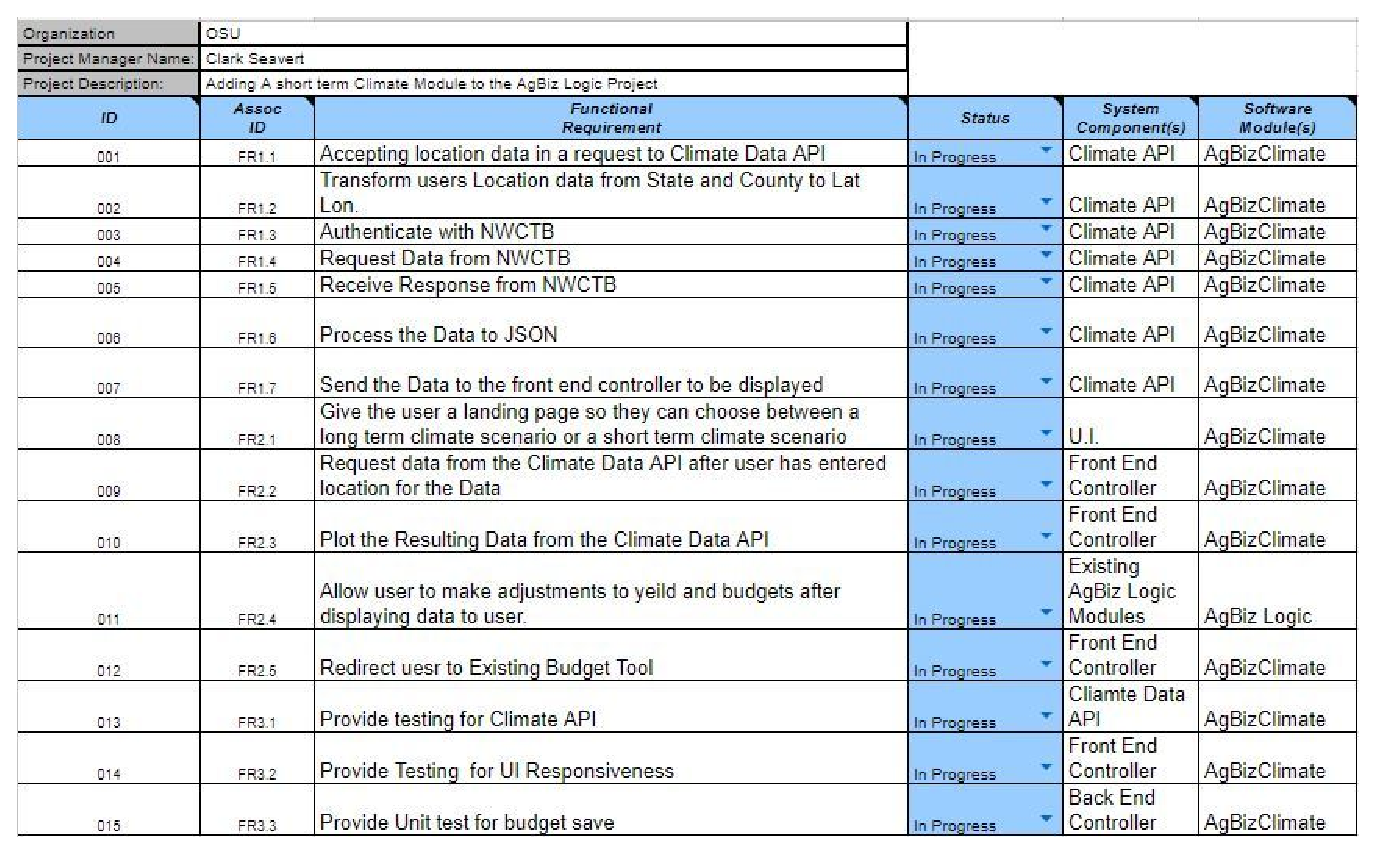
\includegraphics[width=500pt]{Figures/RequirementsMatrix.eps}
			\end{center}
			\caption{Requirements Matrix}
			\label{fig:ReqMat}
		\end{figure}


\end{document}
